% Version 5.0, 2 January 2020

% This tex file can be compiled with
% tectonic templateV5.tex
% https://tectonic-typesetting.github.io
%
% Or simply with the Overleaf latexmkrc configuration: (included in the repo)
% https://www.overleaf.com/learn/how-to/How_does_Overleaf_compile_my_project%3F
%
% A latexindent.yml config file is also included for easier and more consistent
% formatting.

% %%%%%%%%%%%%%%%%%%%%%%%%%%%%%%%%%%%%%%%%%%%%%%%%%%%%%%%%%%%%%%%%%%%%%%%%%%%%%%%%%%%%%%
% TemplateV5.tex -- LaTeX-based template for submissions to the American Meteorological
% Society
% %%%%%%%%%%%%%%%%%%%%%%%%%%%%%%%%%%%%%%%%%%%%%%%%%%%%%%%%%%%%%%%%%%%%%%%%%%%%%%%%%%%%%%
% PREAMBLE
% %%%%%%%%%%%%%%%%%%%%%%%%%%%%%%%%%%%%%%%%%%%%%%%%%%%%%%%%%%%%%%%%%%%%%%%%%%%%%%%%%%%%%%

% Start with one of the following: DOUBLE-SPACED VERSION FOR SUBMISSION TO THE AMS
% \documentclass{ametsocV5}

% TWO-COLUMN JOURNAL PAGE LAYOUT---FOR AUTHOR USE ONLY
\documentclass[twocol]{ametsocV5}

% Enter packages here. If too many math alphabets are used, remove unnecessary packages
% or define hmmax and bmmax as necessary.
%\newcommand{\hmmax}{0}
%\newcommand{\bmmax}{0}
\usepackage{amsmath,amsfonts,amssymb,bm}
\usepackage[british]{babel}
\usepackage{mathptmx}% {times}
\usepackage{newtxtext}
\usepackage{newtxmath}
\usepackage[version=4]{mhchem}
\usepackage[acronym]{glossaries}
\usepackage{cleveref}
\usepackage{siunitx}
\usepackage{listings}
% \usepackage{hyperref}

\makeglossaries{}
\newacronym{agcm}{AGCM}{Atmosphere General Circulation Model}
\newacronym{aodm}{AODVISstdn}{``stratospheric aerosol optical depth 550 nm day night''}
\newacronym{aod}{AOD}{(stratospheric) aerosol optical depth}
\newacronym{aogcm}{AOGCM}{Atmosphere-Ocean General Circulation Model}
\newacronym{c2wmp}{C2W\(-\)}{CESM2(WACCM6) intermediate strength}
\newacronym{c2wm}{C2W\(\downarrow\)}{CESM2(WACCM6) small strength}
\newacronym{c2wsn}{C2WN\(\uparrow\)}{CESM2(WACCM6) large strength, high northern latitude}
\newacronym{c2ws}{C2W\(\uparrow\)}{CESM2(WACCM6) large strength}
\newacronym{c2w}{C2W}{CESM2(WACCM6) tropical}
\newacronym{cam5}{CAM5}{Community Atmosphere Model Version 5}
\newacronym{cam6}{CAM6}{Community Atmosphere Model Version 6}
\newacronym{cesm1}{CESM1}{Community Earth System Model Version 1}
\newacronym{cesm2}{CESM2}{Community Earth System Model Version 2}
\newacronym{cesm}{CESM}{Community Earth System Model}
\newacronym{cice}{CICE5}{CICE Version 5.1.2}
\newacronym{cime}{CIME}{Common Infrastructure for Modelling the Earth}
\newacronym{cism}{CISM2}{Community Ice Sheet Model Version 2.1}
\newacronym{clm}{CLM5}{Community Land Model Version 5}
\newacronym{ecs}{ECS}{equilibrium climate sensitivity}
\newacronym{erf}{ERF}{effective radiative forcing}
\newabbreviation{ob16}{OB16}{\citet{ottobliesner2016}}
\newacronym{esm}{ESM}{Earth System Model}
\newacronym{flnt}{FLNT}{``net longwave flux at the top of the model''}
\newacronym{fpp}{FPP}{Filtered Poisson Process}
\newacronym{fsnt}{FSNT}{``net solar flux at the top of the model''}
\newacronym{fsst}{\texttt{fSST1850}}{fixed sea-surface temperature}
\newacronym{irf}{IRF}{instantaneous radiative forcing}
\newacronym{lwcf}{LWCF}{``long wave cloud forcing''}
\newacronym{lw}{LW}{long wave}
\newacronym{mam3}{MAM3}{three mode version of the Modal Aerosol Module}
\newacronym{mam}{MAM}{Modal Aerosol Module}
\newacronym{marbl}{MARBL}{MARine Biogeochemistry Library}
\newacronym{ma}{MA}{middle atmosphere}
\newacronym{mosart}{MOSART}{MOdel for Scale Adaptive River Transport}
\newabbreviation{j05}{J05}{\citet{jones2005}}
\newabbreviation{g16}{G16}{\citet{gregory2016}}
\newabbreviation{m20}{M20}{\citet{marshall2020dataset}}
\newabbreviation{t10}{T10}{\citet{timmreck2010}}
\newabbreviation{n15}{N15}{\citet{niemeier2015}}
\newacronym{pop}{POP2}{Parallel Ocean Program Version 2}
\newacronym{qbo}{QBO}{quasi-biennial oscillation}
\newacronym{rf}{RF}{(effective) radiative forcing}
\newacronym{swcf}{SWCF}{``short wave cloud forcing''}
\newacronym{sw}{SW}{short wave}
\newacronym{tcrp}{TCRP}{transient climate response parameter}
\newacronym{toa}{TOA}{top-of-the-atmosphere}
\newacronym{trefht}{TREFHT}{``reference height temperature''}
\newacronym{waccm}{WACCM6}{Whole Atmosphere Community Climate Model Version 6}
\newacronym{ww3}{WW3}{Wave Watch Version 3}
\newacronym{ytt}{YTT}{Young Toba Tuff}


% Create some cusotm commands
\newcommand{\iso}[1][i]{{#1}njected \ce{SO2}}

% %%%%%%%%%%%%%%%%%%%%%%%%%%%%%%%%%%%%%%%%%%%%%%%%%%%%%%%%%%%%%%%%%%%%%%%%%%%%%%%%%%%%%%

% To be entered by author:
% May use \\ to break lines in title:
\title{
  Parameter Scan: Volcanic influence on climate across multiple magnitudes and injected
  altitudes
}

% Enter authors' names, as you see in this example: Use \correspondingauthor{} and
% \thanks{Current Affiliation:...} immediately following the appropriate author. Note
% that the \correspondingauthor{} command is NECESSARY. The \thanks{} commands are
% OPTIONAL.

\authors{
  Eirik Rolland Enger\correspondingauthor{Eirik Rolland Enger, eirik.r.enger@uit.no}
}

% Follow this form: \affiliation{American Meteorological Society, Boston, Massachusetts}
\affiliation{UiT The Arctic University of Norway, Tromsø, Norway}

% \affiliation{}

% If appropriate, add additional authors, different affiliations:
\extraauthor{Audun Theodorsen}
\extraaffil{UiT The Arctic University of Norway, Tromsø, Norway}
\extraauthor{Rune Graversen}
\extraaffil{UiT The Arctic University of Norway, Tromsø, Norway}
\extraauthor{Martin Rypdal}
\extraaffil{UiT The Arctic University of Norway, Tromsø, Norway}
\extraauthor{Maria Rugenstein}
\extraaffil{Colorado State University, Fort Collins, Colorado}

% %%%%%%%%%%%%%%%%%%%%%%%%%%%%%%%%%%%%%%%%%%%%%%%%%%%%%%%%%%%%%%%%%%%%%%%%%%%%%%%%%%%%%%
% ABSTRACT
%
% Enter your abstract here. Abstracts should not exceed 250 words in length!

\abstract{
  Volcanoes affect Earth's climate. What happens when the climate is forced with
  volcanoes of different size and injected at different heights? Should we expect to see
  the same climate response for the same volcanoes in a different, warmer climate?
}

\begin{document}

% Necessary!
\maketitle

% %%%%%%%%%%%%%%%%%%%%%%%%%%%%%%%%%%%%%%%%%%%%%%%%%%%%%%%%%%%%%%%%%%%%%%%%%%%%%%%%%%%%%%
% SIGNIFICANCE STATEMENT/CAPSULE SUMMARY
% %%%%%%%%%%%%%%%%%%%%%%%%%%%%%%%%%%%%%%%%%%%%%%%%%%%%%%%%%%%%%%%%%%%%%%%%%%%%%%%%%%%%%%
%
% If you are including an optional significance statement for a journal article or a
% required capsule summary for BAMS (see
% www.ametsoc.org/ams/index.cfm/publications/authors/journal-and-bams-authors/formatting-and-manuscript-components
% for details), please apply the necessary command as shown below:
%
% \statement
% Significance statement here.
%
% \capsule
% Capsule summary here.

% %%%%%%%%%%%%%%%%%%%%%%%%%%%%%%%%%%%%%%%%%%%%%%%%%%%%%%%%%%%%%%%%%%%%%%%%%%%%%%%%%%%%%%
% MAIN BODY OF PAPER
% %%%%%%%%%%%%%%%%%%%%%%%%%%%%%%%%%%%%%%%%%%%%%%%%%%%%%%%%%%%%%%%%%%%%%%%%%%%%%%%%%%%%%%

% In all cases, if there is only one entry of this type within the higher level heading,
% use the star form:
%
% \section{Section title}
% \subsection*{subsection}
% text...
% \section{Section title}
%
% vs
%
% \section{Section title}
% \subsection{subsection one}
% text...
% \subsection{subsection two}
% \subsubsection{First tertiary heading}
% \paragraph{First quaternary heading}
% \section{Section title}

\section{Outline}

The paper should provide insight about what might happen if a large (order of magnitude
or more than Mount Pinatubo) volcano erupted (for example within the next 50 years).
\emph{Little literature can be found that investigate the effects of eruptions ten times
  or more than that of Mount Pinatubo, so this should hopefully be worthwhile looking
  into.} It should also be about how volcanic simulations compare in magnitude and model
complexity (dynamic ocean against slab ocean). If there is no big difference, we may
also run more experiments to test for other things:
\begin{itemize}
  \item How does the climate response change based on the state of the climate: what if we run a
        \ce{CO2} doubling or quadrupling simulation until close to equilibrium, and let the
        volcanoes erupt then?
  \item How much does it matter how high in the atmosphere the initial \ce{SO2} is injected?
  \item How far does the linear relation between \acrshort{aod} and \acrshort{toa} go?
\end{itemize}

\subsection*{Introduction}

The introduction should go into some detail about:

\begin{itemize}
  \item Importance of volcanic eruptions for temperature fluctuations
  \item Refer back to other simulations of volcanoes, for example the \citet{jones2005} paper
        that ran a super-volcano, or \citet{gregory2016} who looked at historic volcanoes during
        the last 150 years only
  \item The temperature response might be more sensitive to the sign of the forcing, rather than
        the forcing agent, and as such a halving of \ce{CO2} may be compared with volcanoes
        \citep{gunther2022}
  \item How important is it that \ce{SO2} is injected at a given height?
  \item To some extent there should be a literature review of the above, so more citations and
        references are needed.
\end{itemize}

\subsection*{References}

\begin{description}
  \item[overview] \citet{marshall2022}
  \item[feedback params] \citet{boer2007, gunther2022, gregory2020, hansen2005, knutti2017,
      marvel2016, merlis2014, ollila2016, pauling2021, richardson2019, salvi2022, wigley2005}
  \item[climate impact] \citet{gregory2016, jones2005, ottobliesner2016, santer2016,
      timmreck2009, timmreck2010, toohey2016b, yang2019, yokohata2005, zanchettin2019}
  \item[eruptions] \citet{arfeuille2014, douglass2006, lin2022, marshall2019, marshall2020,
      marshall2021, schmidt2018, soden2002, sukhodolov2018}
  \item[other phenomena] \citet{chen2022, lehner2016, marshall2018}
  \item[models] \citet{rypdal2012}
  \item[cesm2] \citet{danabasoglu2020, gettleman2019, lawrence2019, li2013, liu2016, mills2016,
      smith2010}
\end{description}

\citet{marshall2022} mention (in the graphic in their figure 1) that the \emph{role of
  initial conditions} is a key outstanding question. This could be a contribution to
that. Also, when aerosols grow, they scatter radiation less efficiently and also fall
down faster, so the temperature response should be damped for increasing eruption
magnitude. Clustering and long term effects are mentioned in its own section
(Multi-decadal impacts) along with the dependence of the current climate state.

\citet{marshall2019} does many similar things to what I have done, but do not focus on
seasonal variability. This is however mentioned as one other direction to dig into, and
is somewhat covered by \citet{marshall2020}. Assumes that there is an $e$-folding time,
but notes that it does change, so they calculate an average time over a small range
(from a month after the peak until you reach ten percent of the peak). They further note
that the $e$-folding time is dependent on latitude mostly, but also on injected
\ce{SO2}. Their eruptions all occur in July, thus winter (February) can be a possible
avenue (nope, this is covered by \citet{marshall2020}, which uses the \(41\) simulations
from \citet{marshall2019}, as well as the exact same ones but starting on 1 January
instead of 1 July). This would be hard or likely not possible to answer without creating
an emulator myself, for which I have too few simulations.

In \citet{marshall2020}, they take the reconstructed \acrshort{saod} from
\citet{toohey2017}, convert it to radiative forcing based on their conversions, and plot
the corresponding temperature time series from each radiative forcing using a simple
climate model. So, can we use this with the \acrfull{fpp} framework?

Perhaps focus on why there seems to be a loop in the \acrshort{aod} against
\acrshort{toa} plots. Can also compare February-August means with May-November means.
(\citet{marshall2021} discuss Tambora, but mention that it erupted in April, while their
data consist of January and July eruptions.)

% TODO: we should have a section for method as well, and maybe also write about what the
% results and discussion should include

\section{Method}

\subsection{Model}

We are using the \acrfull{cesm2} \citep{danabasoglu2020} to run our climate simulations,
together with the \acrfull{waccm} \citep{gettleman2019}. \acrshort{cesm2} is run with
the full dynamical ocean component \acrfull{pop} \citep{smith2010, danabasoglu2020}, as
well as having \acrfull{mosart} \citep{li2013, danabasoglu2020}, \acrfull{clm}
\citep{lawrence2019, danabasoglu2020}, \acrfull{ww3}, \acrfull{cice}, \acrfull{cism} and
\acrfull{cime} included.

The model atmosphere was run at nominal \(\SI{2}{\degree}\) resolution, with \(70\)
vertical levels, in the \acrfull{ma} configuration.

The \acrshort{ma} version of \acrshort{waccm} uses the \acrfull{mam3}
\citep{gettleman2019}. This was made as a simplified and computationally efficient
default setting in the \acrshort{cam5} \citep{liu2016}, and is described in
\citet{liu2012}. The \acrshort{mam3} was created from MAM7 (seven modes) by merging the
primary carbon mode with the accumulation mode, and assuming instantaneous internal
mixing of primary carbonaceous aerosols with secondary aerosols \citep{liu2016}.
Specifically, the three modes are Aitken, accumulation and coarse (MAM7 includes Aitken,
accumulation, primary carbon, fine dust and fine sea salt, coarse dust and coarse sea
salt modes) \citep{liu2016}. Instantaneous ageing of primary carbonaceous particles is
assumed by emitting them in the accumulation mode. There are \( 15 \) transported
aerosol tracers in \acrshort{mam3} \citep{liu2016}. (\citet{marshall2019, marshall2020,
  marshall2021} used a code with seven log-normal modes to simulate aerosol mass and
number concentrations, but their model is an \acrfull{agcm}, as opposed to the
\acrshort{cesm2} which is an \acrfull{esm} or \acrfull{aogcm}.)

\subsection{Simulation set up}

Simulations was created using a modified version of
\url{http://svn.code.sf.net/p/codescripts/code/trunk/ncl/emission/createVolcEruptV3.ncl}
% \href{http://svn.code.sf.net/p/codescripts/code/trunk/ncl/emission/createVolcEruptV3.ncl}{\texttt{createVolcEruptV3.ncl}}
file, via a Python project developed on GitHub:
\url{https://github.com/engeir/volcano-cooking}, which is also available from the Python
package manager PyPI, as \texttt{pip install volcano-cooking}. This creates volcanoes
with a given \ce{SO2} amount that is injected over six
hours\footnote{\url{http://svn.code.sf.net/p/codescripts/code/trunk/ncl/emission/createVolcEruptV3.ncl}}
at a given altitude and latitude, longitude. All volcanic \ce{SO2} files are created by
setting the eruption details in a \texttt{JSON} file that is read to the
\texttt{volcano-cooking} CLI at a specified version, making the experiment setup easy to
reproduce.

We are using the \texttt{BWma1850} component setup to run the \acrshort{cesm2}, and an
accompanying \acrfull{fsst} simulation to obtain estimates of the radiative forcing. The
\acrshort{fsst} that is run is not a standardised component setup as of \acrshort{cesm2}
(v2.1.3), but is instead specified in full as (\texttt{BWma1850} full name also shown
for reference)
\begin{small}
  \begin{verbatim}
BWma1850 ->
  1850_CAM60%WCCM_CLM50%BGC-CROP_CICE_
  POP2%ECO%NDEP_MOSART_CISM2%NOEVOLVE_WW3
fSST1850 ->
  1850_CAM60%WCCM_CLM50%BGC-CROP_CICE%PRES_
  DOCN%DOM_MOSART_CISM2%NOEVOLVE_SWAV_TEST
  \end{verbatim}
\end{small}
They differ in \texttt{CICE -> CICE\%PRES}, which is prescribed sea-ice,
\texttt{POP2\%ECO\%DEP -> DOCN\%DOM} which is from a dynamical ocean to a prescribed
data ocean and the wave component \texttt{WW3 -> SWAV} which is now a stub wave
component.

\subsection{Simulations}

The simulations cover three \ce{SO2} injection magnitudes and four seasons; 15 February,
15 May, 15 August and 15 November. The magnitudes vary across three orders of magnitude:
\(\SI{26}{\tera\gram}\), \(\SI{400}{\tera\gram}\) and \(\SI{1629}{\tera\gram}\). The
smallest eruption is of the same order of magnitude as Mount Pinatubo
\citep[\(\sim10\)--\(\SI{20}{\tera\gram}\);~e.g.,][]{timmreck2018} and Mount Tambora
\citep[\(\sim\SI{56.2}{\tera\gram}\);~e.g.,][]{zanchettin2016}, the intermediate is
similar to the 1257 Samalas eruption
\citep[\(\sim\SI{119}{\tera\gram}\);][]{toohey2017}, and the largest is similar to the
Young Toba Tuff eruption
\citep[\(10\)--\(\SI{10000}{\tera\gram}\);][and~references~therein]{jones2005}. They are
all located at the equator, at \(\SI{0}{\degree N}\), \(\SI{1}{\degree E}\).

\section{Results}

\subsection{Figures}

Let us now introduce some figures.

\paragraph{Forcing magnitudes}

There are the three different forcing magnitudes that have been used. The figures below
show two alternative ways of normalizing the temperature response to these volcanic
events.

First, we have the three temperature responses normalized by setting the peak value
equal to one, shown in \cref{fig:temp_norm_max}. The second method of normalizing, shown
in \cref{fig:temp_norm_int}, is to numerically integrate the time series, and divide
through such that they integrate to one.

When normalizing by setting their amplitude equal to (minus) one, the initial rise
across all three is comparable. The difference among the three is how much more quickly
the temperature reverts back to equilibrium in the smallest eruption case.

On the other hand, when normalizing by enforcing all to integrate to the same value, the
tail where the temperature revert back is the most similar across all three eruptions.
From these two normalizations, one thing that stays different is the amount of time
spent at the peak temperature. The temperature from smaller eruption simulation starts
to revert sooner after it reaches temperatures close to the peak temperature. The shape
of the initial rise and the tail is more similar across the three.

\begin{figure}
  \begin{center}
    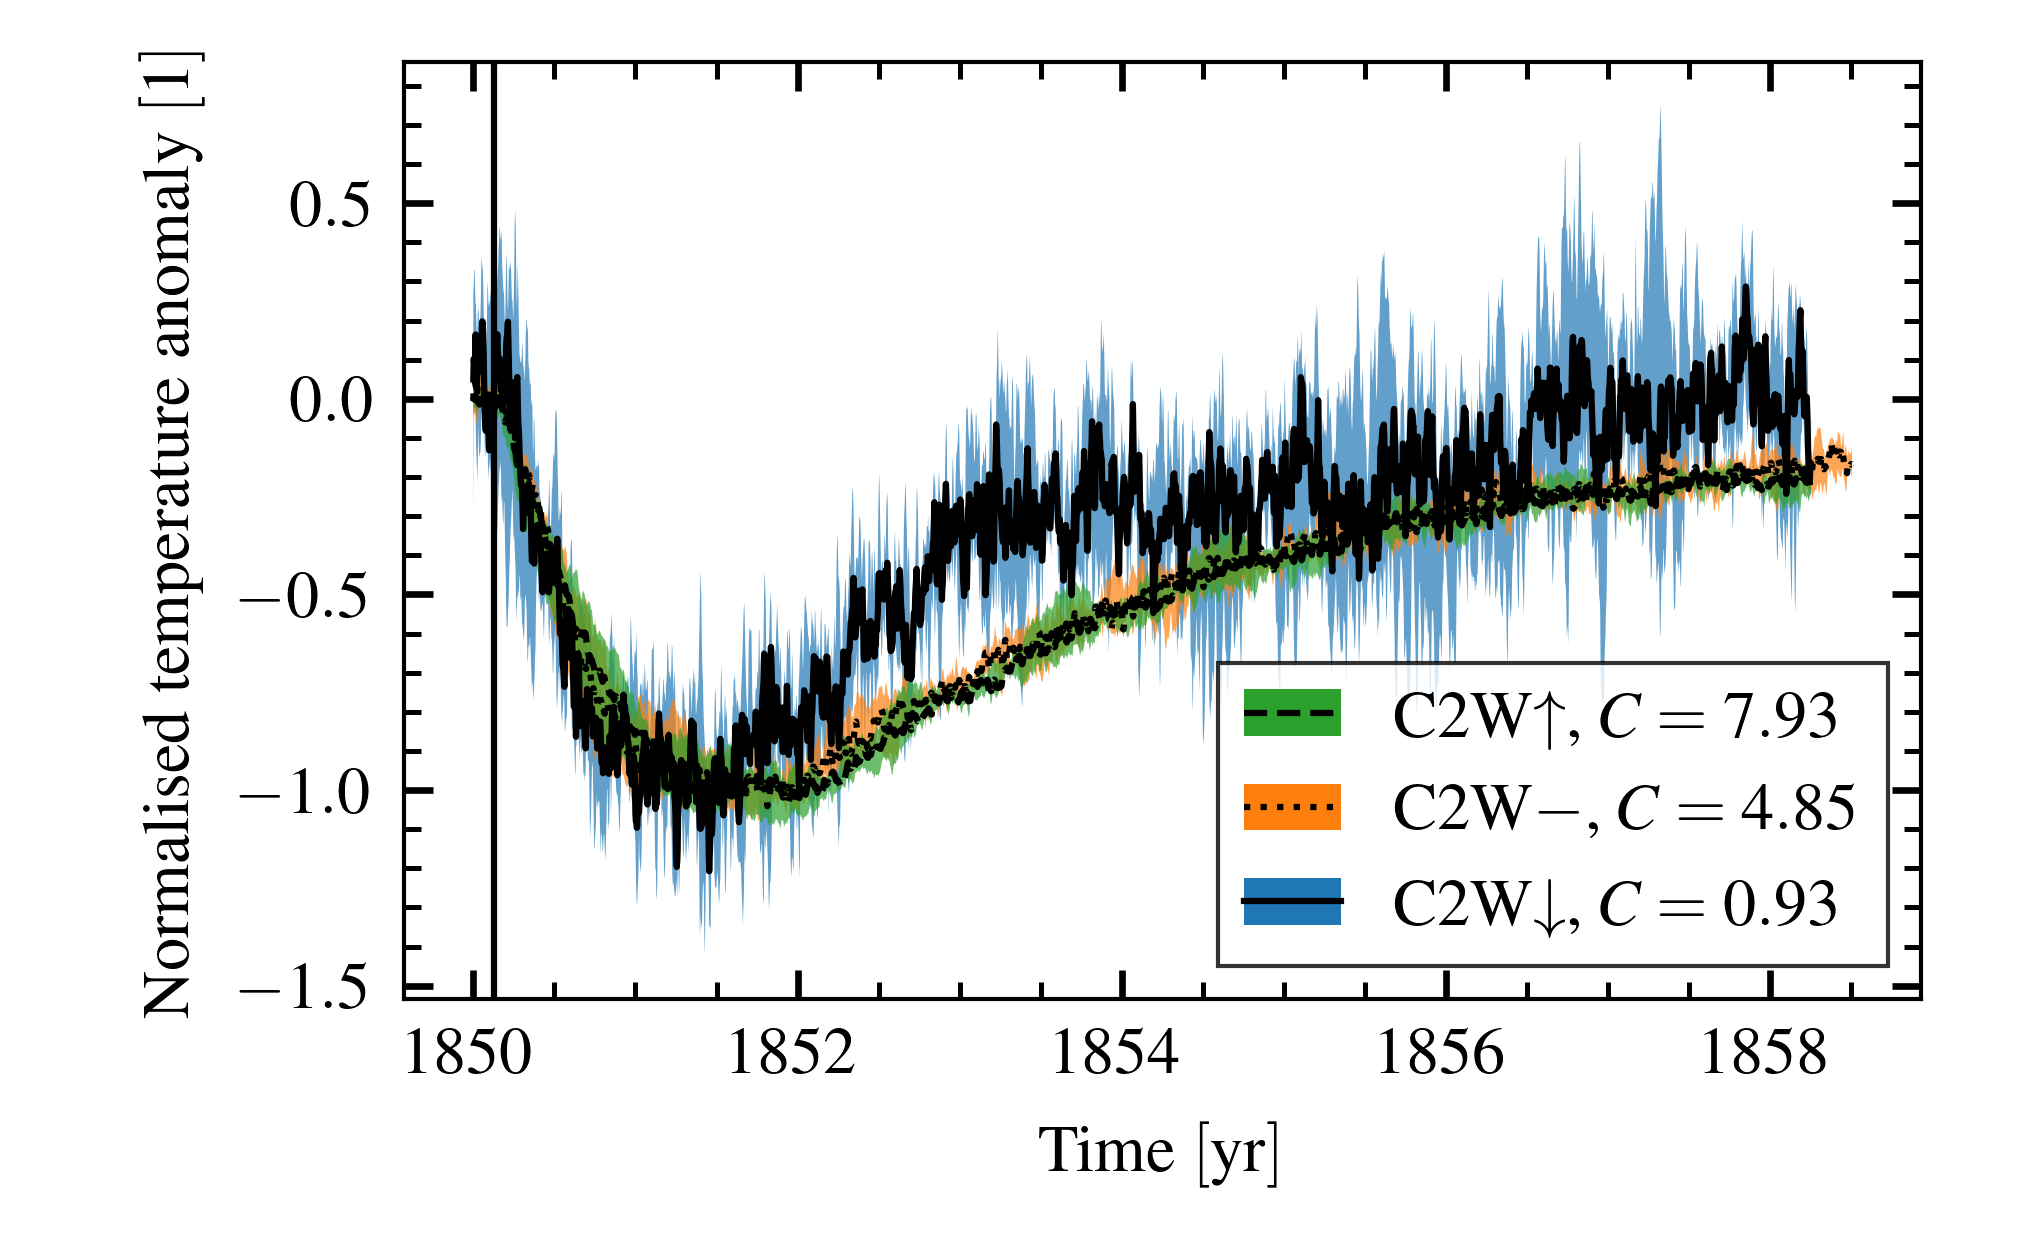
\includegraphics[width=0.95\linewidth]{figures/compare-waveform-max.png}
  \end{center}
  \caption{Normalized temperature response to three different-size volcanic eruptions,
    by setting a maximum peak value}%
  \label{fig:temp_norm_max}
\end{figure}

\begin{figure}
  \begin{center}
    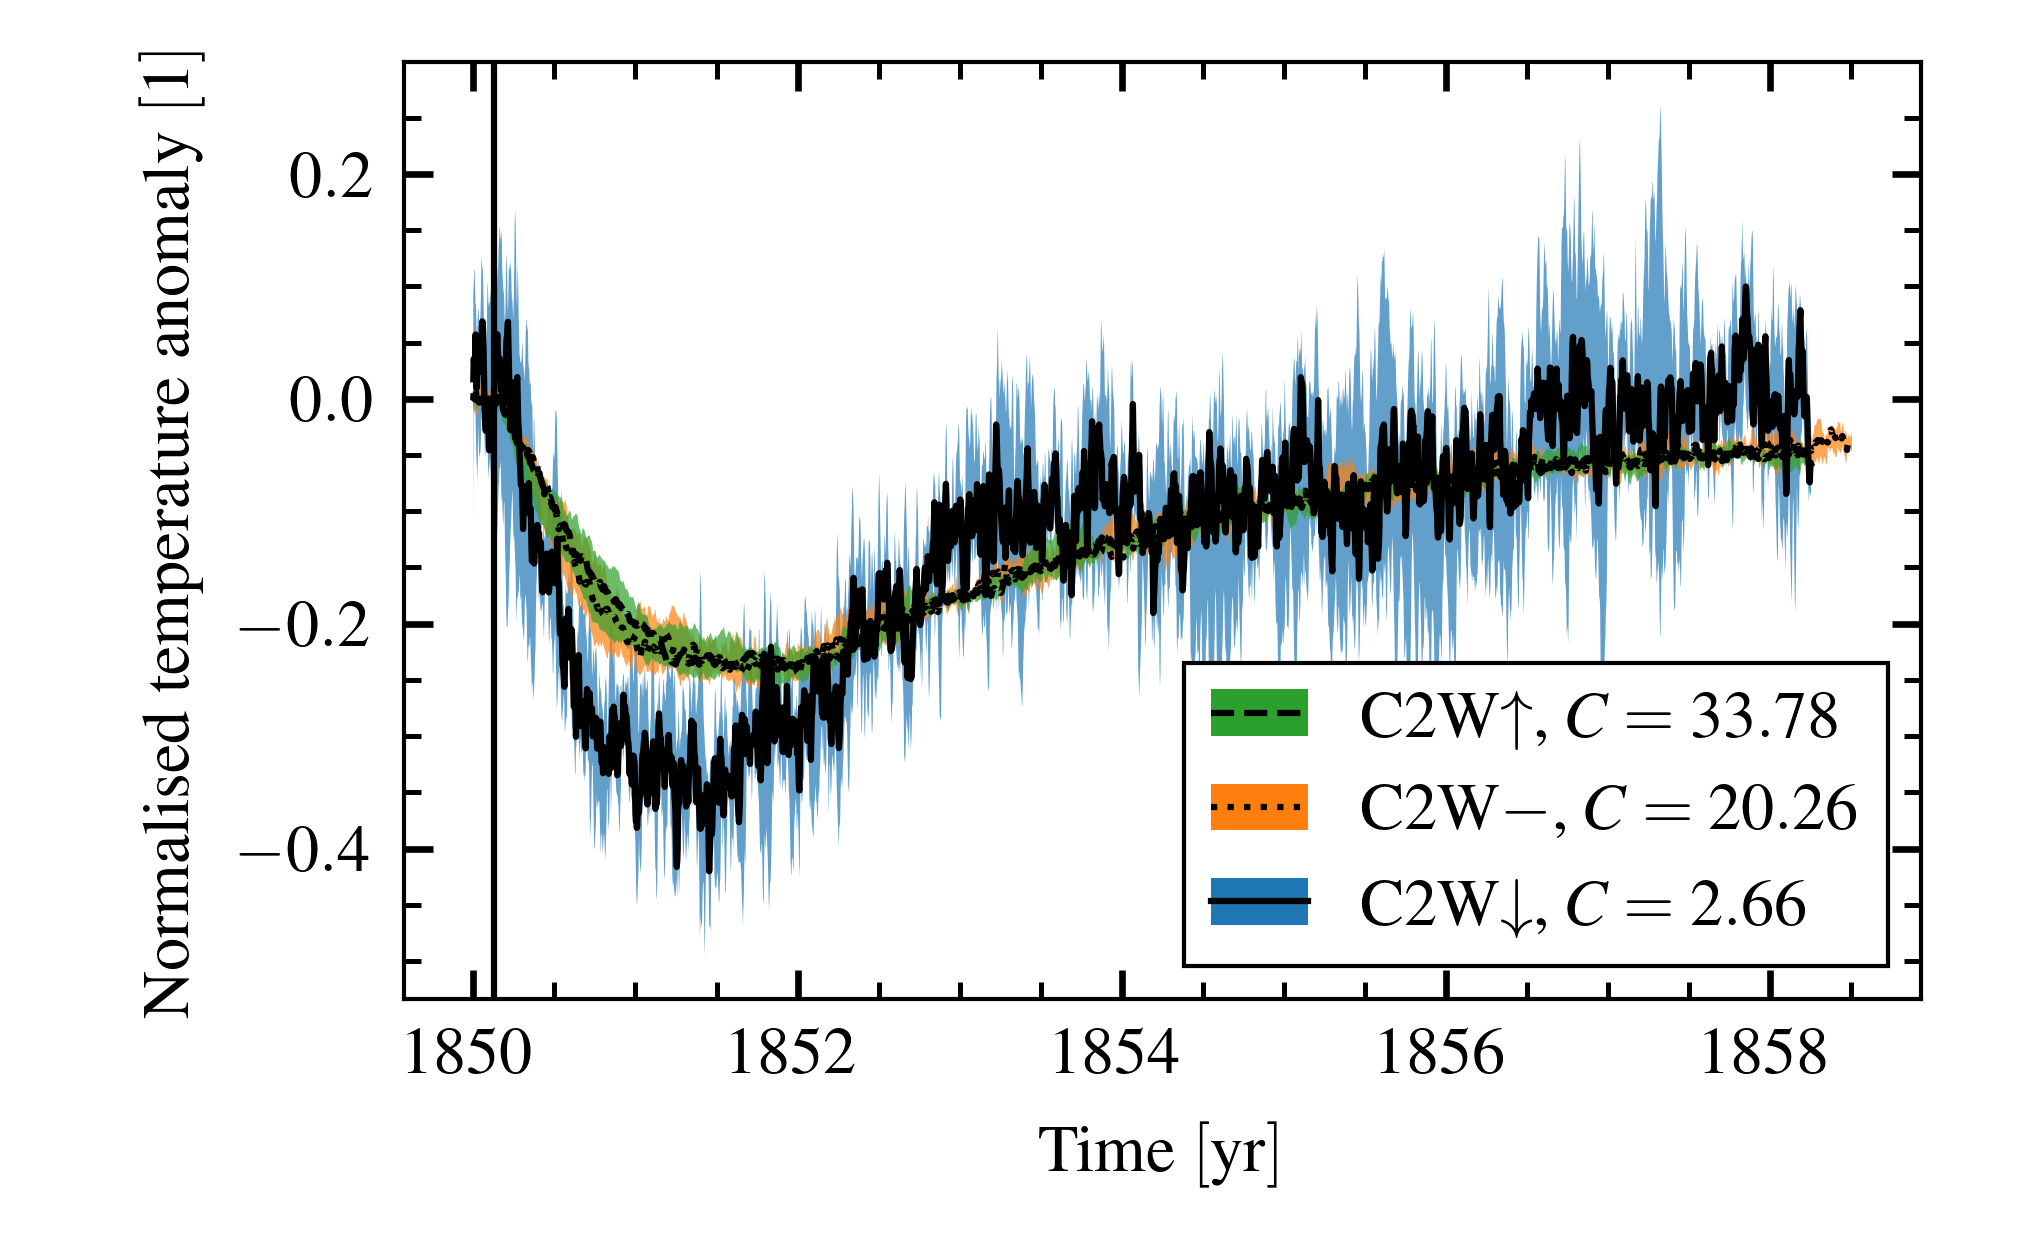
\includegraphics[width=0.95\linewidth]{figures/compare-waveform-integrate.png}
  \end{center}
  \caption{Normalized temperature response to three different-size volcanic eruptions,
    using integration, i.e., they all integrate to one}%
  \label{fig:temp_norm_int}
\end{figure}

\paragraph{Superposing volcanoes}

\emph{See \citet{toohey2016b}.}

Let us now look at how the temperature behave when forced by two eruptions occurring
close in time (four years apart), shown in \cref{fig:double-overlap-superpose}. The
temperature is still perturbed as the second eruption happen, but when comparing this
with the superposition of the temperature time series of two single eruption events,
their alignment is quite good. Therefore, we cannot from this say that the temperature
response is sensitive to overlapping eruptions.

\emph{Can we say anything that relates to other work and how the physics is described?}

Previous work have reported no prolonged or persistent cooling after a double-volcano
event with eruptions four years apart with \ce{SO2} injections of \( \SI{30}{\tera\gram}
\) and \( \SI{50}{\tera\gram} \) \citep{toohey2016b}. This was, however, contrary to
observations based on tree ring width data showing a persistent cooling from the two
eruptions that was simulated.

\begin{figure}
  \begin{center}
    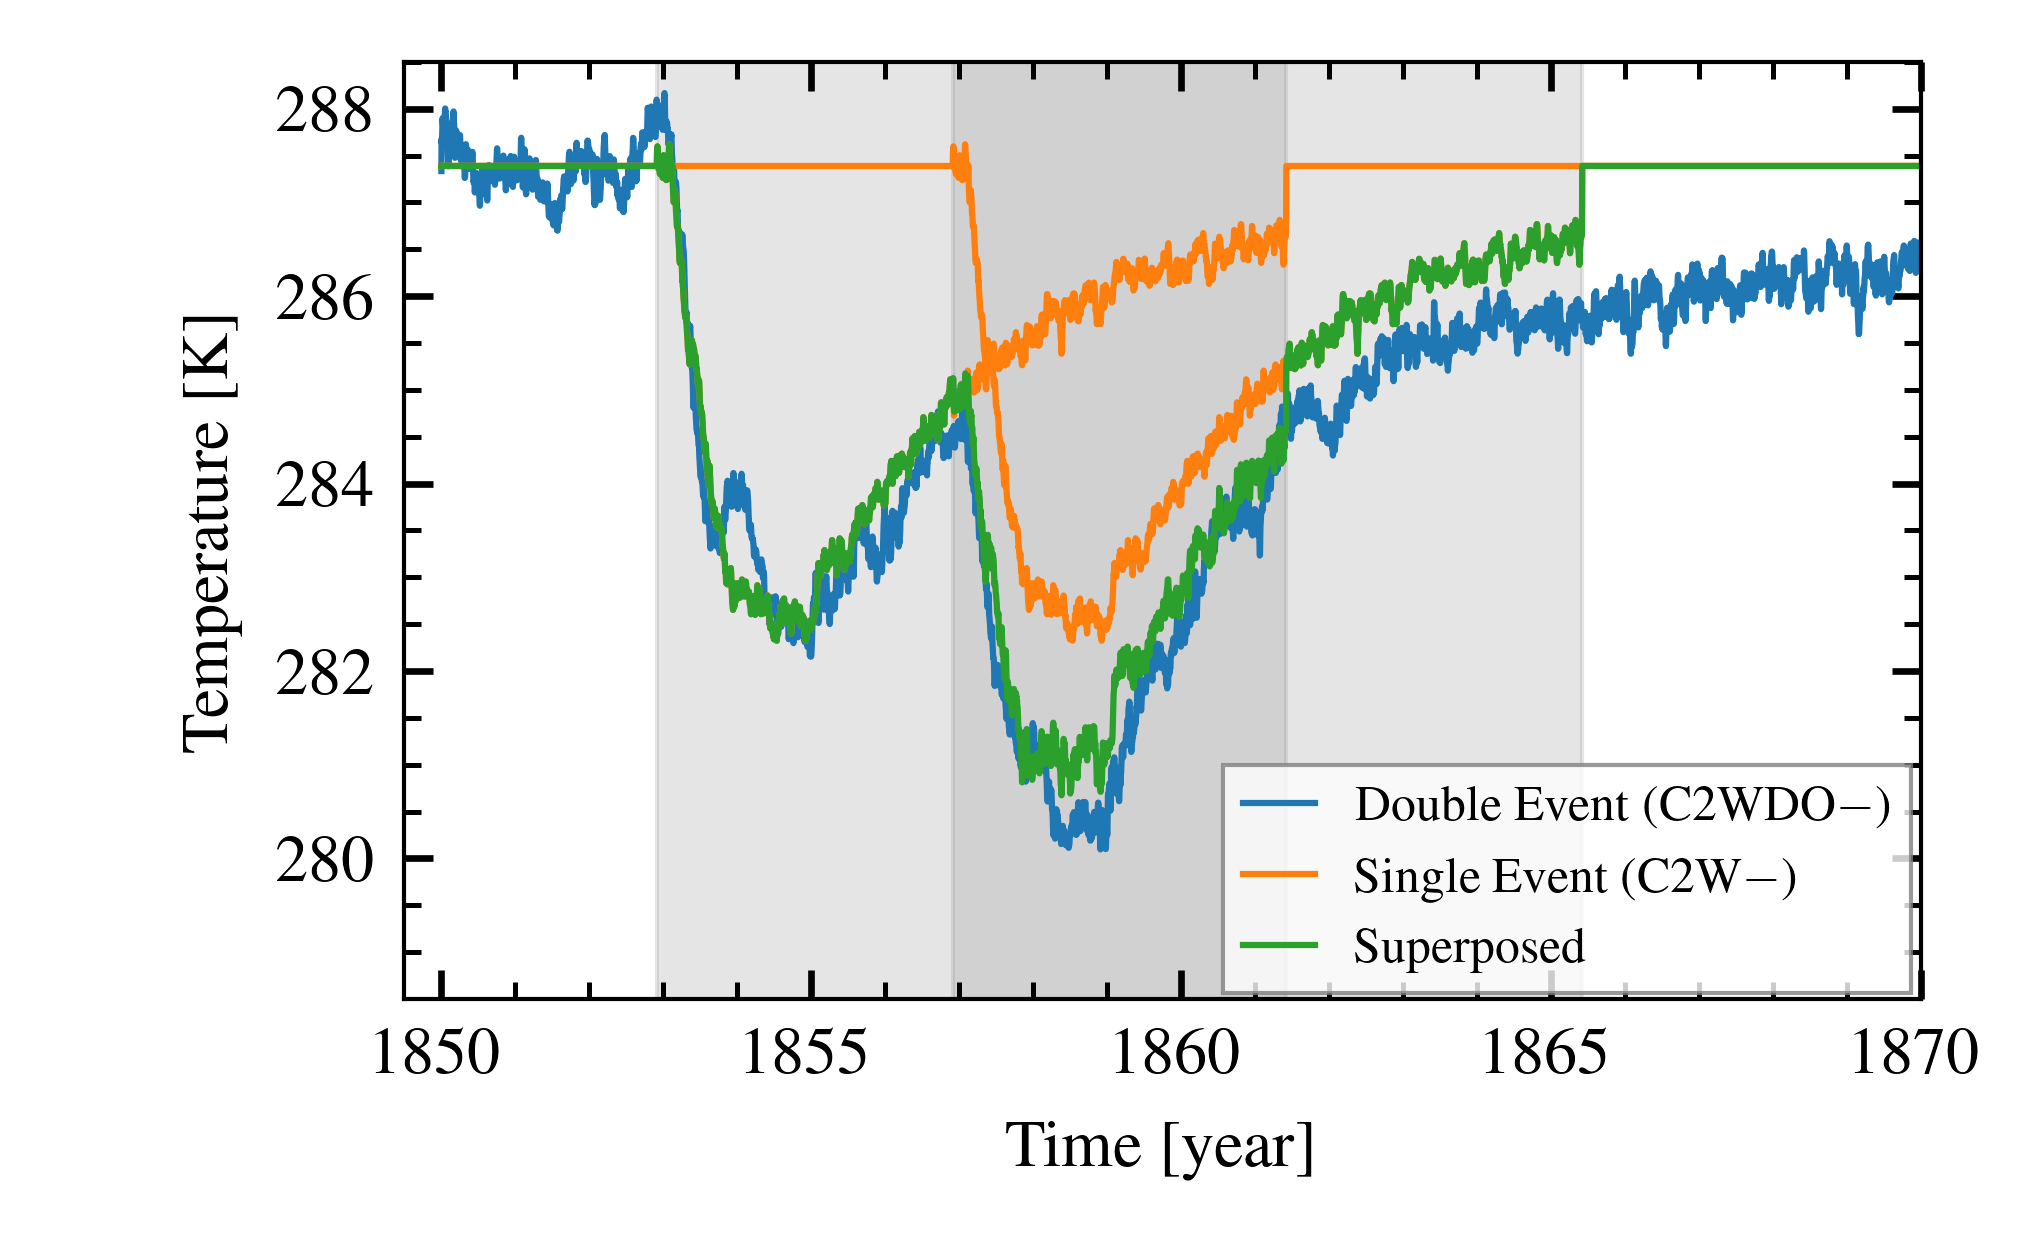
\includegraphics[width=0.95\linewidth]{figures/double-overlap-superpose.png}
  \end{center}
  \caption{Double-eruption event, where the temperature responses from the two eruptions
    overlap. That is, the second equivalent eruption occur as the temperature is still
    perturbed from the first eruption}%
  \label{fig:double-overlap-superpose}
\end{figure}

\paragraph{Parameter scan}

So far we have been focusing on temperature. We here look more closely into the
different forcings as well. This comparison is motivated by \citet{gregory2016},
specifically their figure 4 which compare annual mean aerosol optical depth with
radiative forcing. \Cref{fig:aod_vs_toa_full} show annual mean values from the three
simulation cases along with the gradient obtained by \citet{gregory2016} (\(-19\)).
First off, the \acrshort{toa} values are clearly much smaller compared the
\acrshort{aod} than what was the case for \citet{gregory2016} and the data used in their
figure.

\begin{figure}
  \begin{center}
    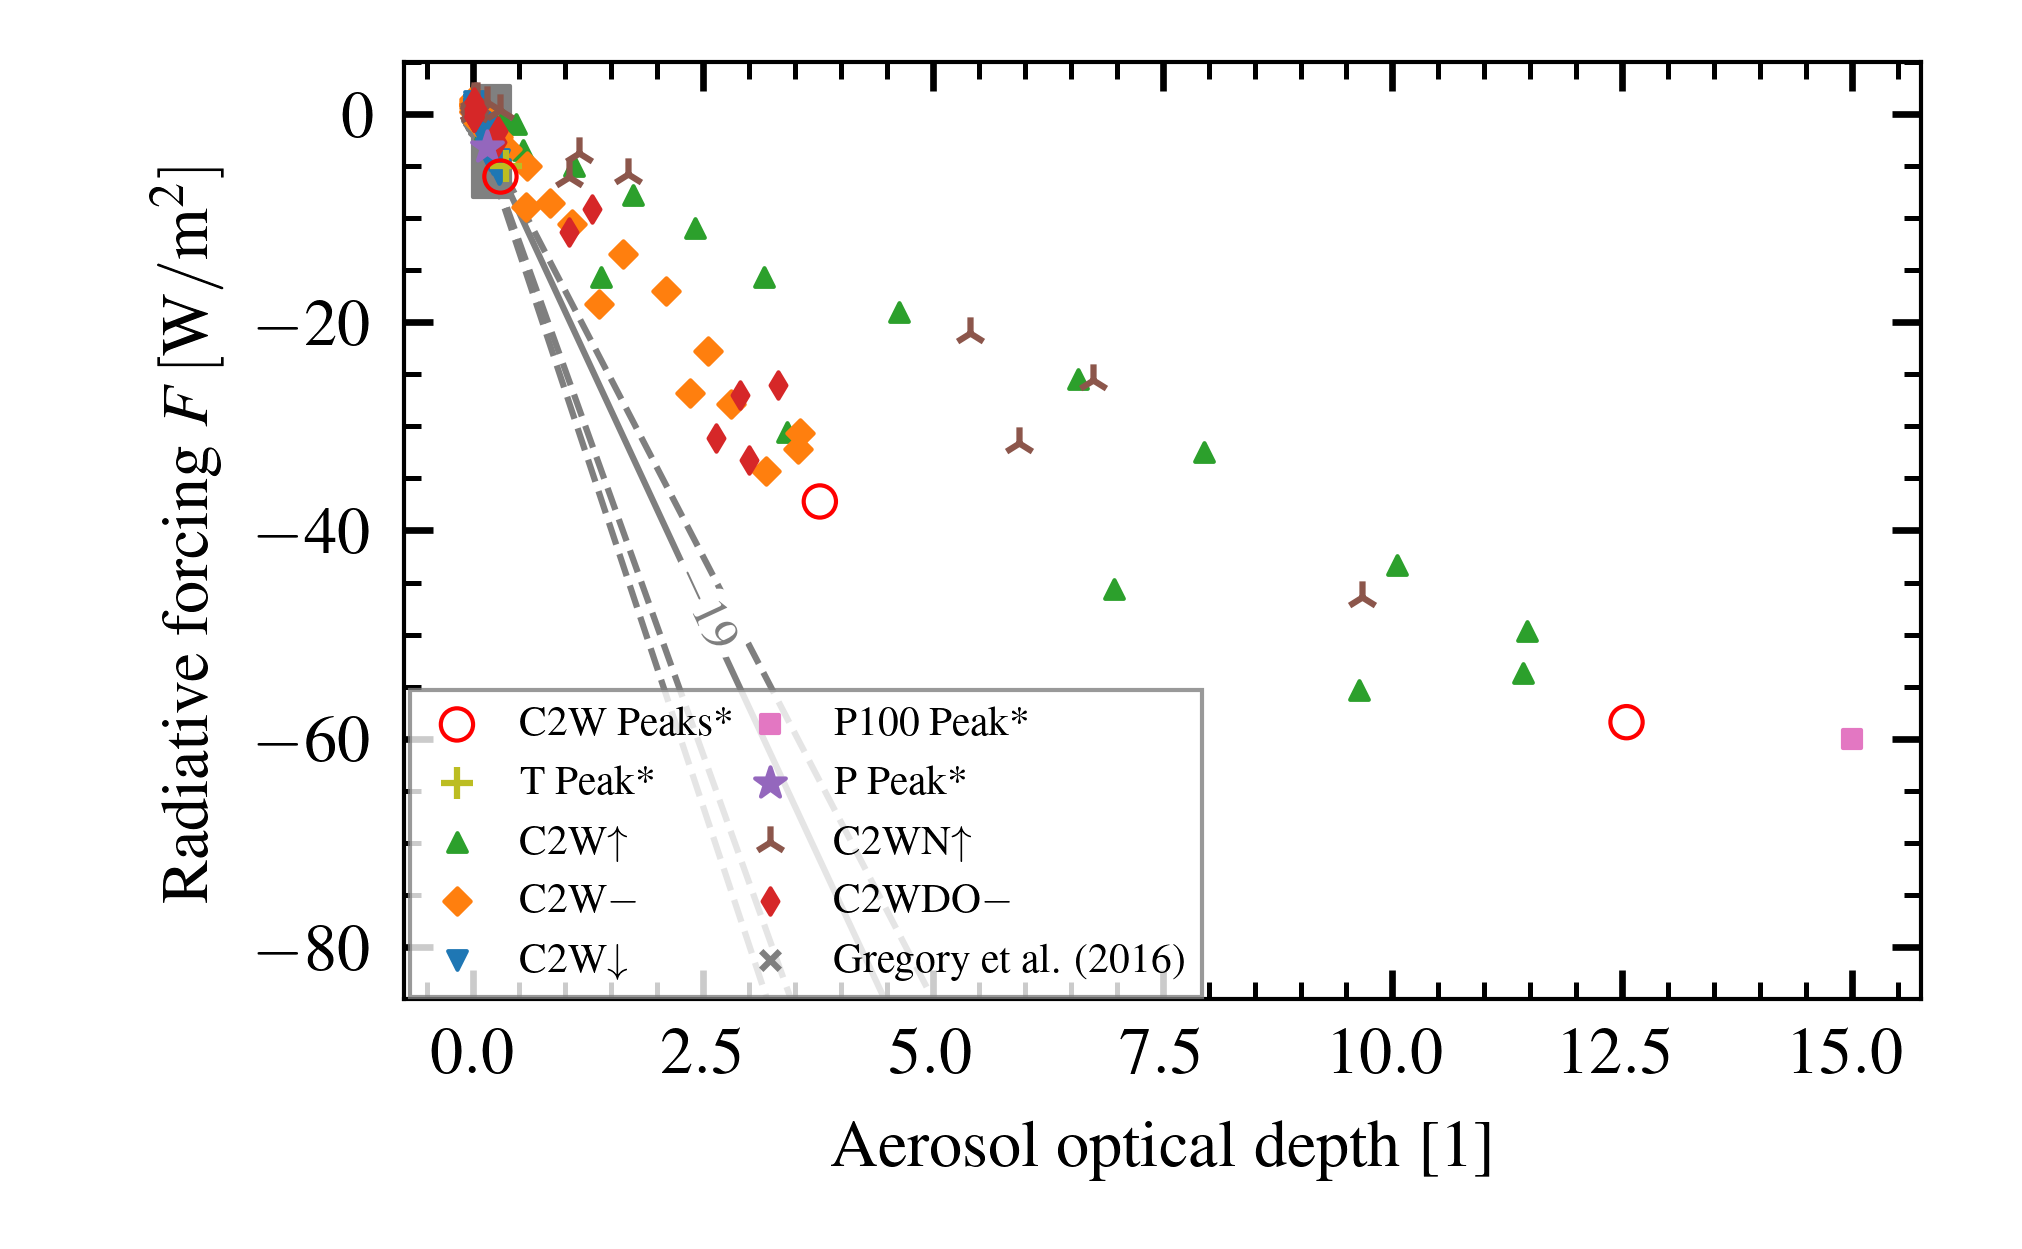
\includegraphics[width=0.95\linewidth]{figures/aod_vs_toa_avg_full.png}
  \end{center}
  \caption{\acrshort{aod} versus \acrshort{toa}, full size. Same type as
    \citet{gregory2016}}%
  \label{fig:aod_vs_toa_full}
\end{figure}

\begin{figure}
  \begin{center}
    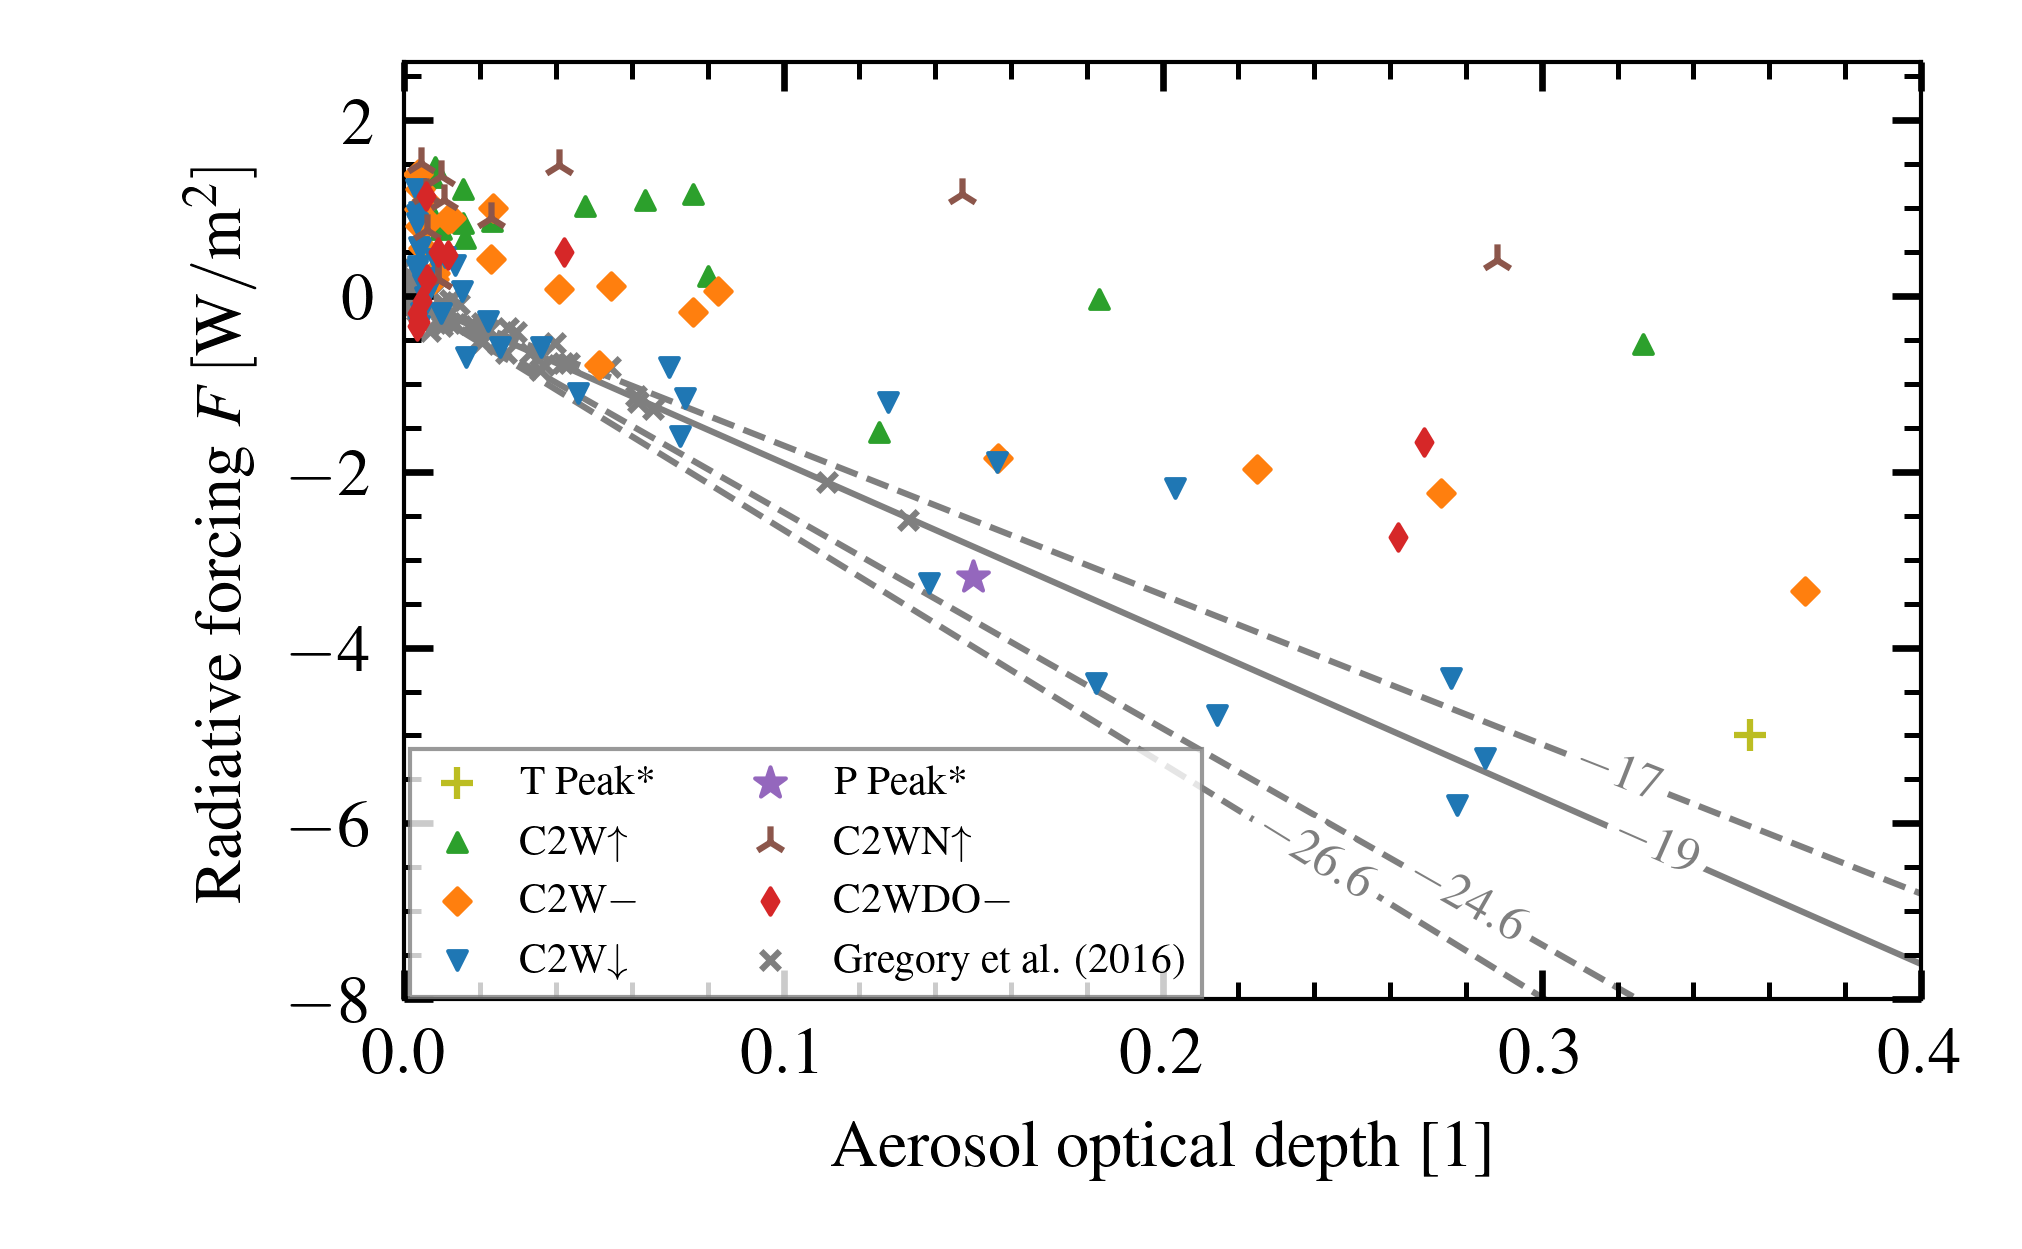
\includegraphics[width=0.95\linewidth]{figures/aod_vs_toa_avg_inset.png}
  \end{center}
  \caption{\acrshort{aod} versus \acrshort{toa}, inset. Same type as
    \citet{gregory2016}}%
  \label{fig:aod_vs_toa_inset}
\end{figure}

\begin{figure}
  \begin{center}
    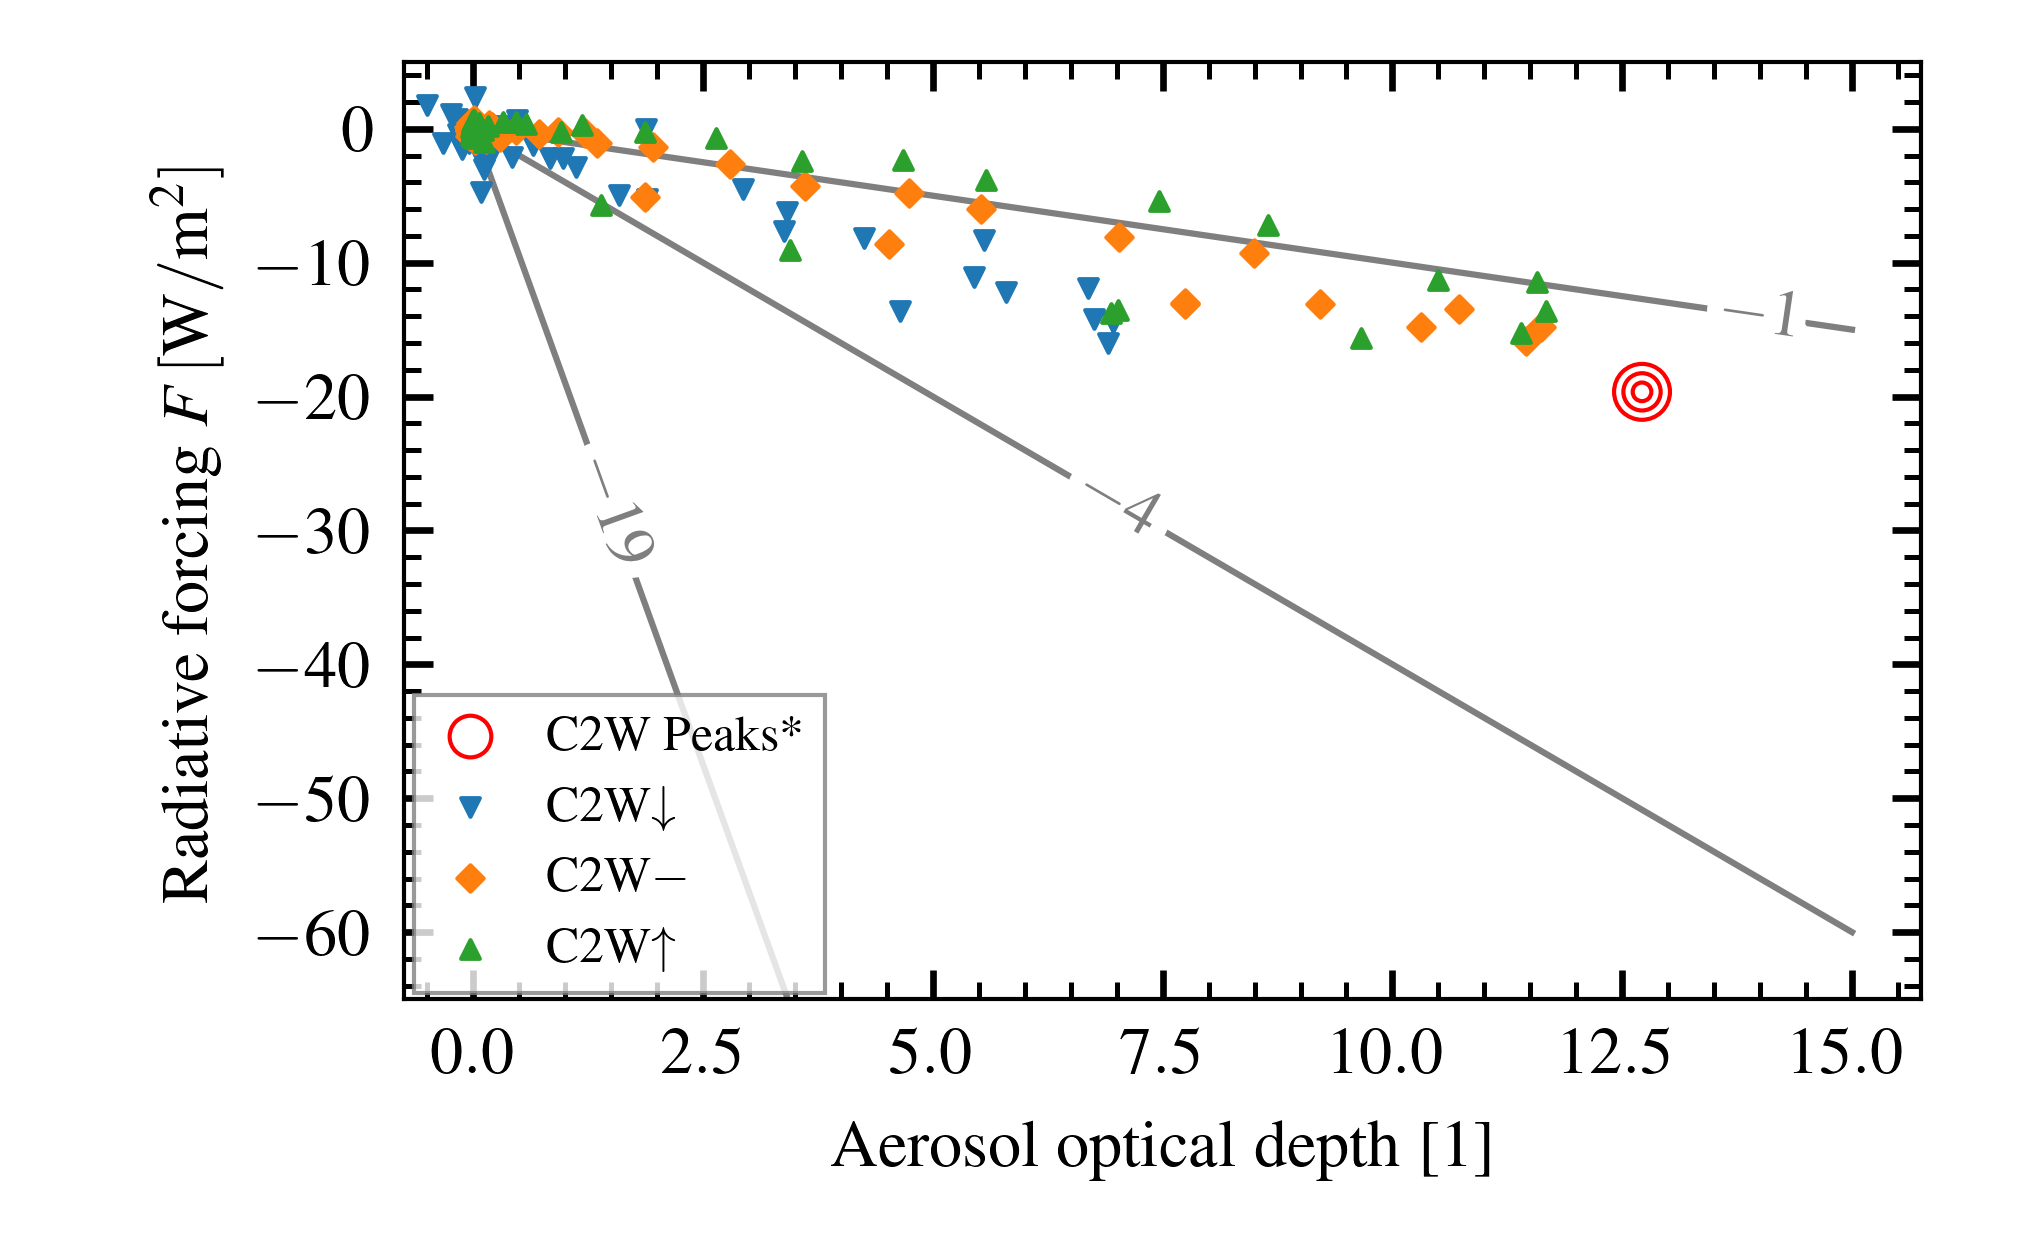
\includegraphics[width=0.95\linewidth]{figures/aod_vs_toa_avg_scaled.png}
  \end{center}
  \caption{
    \acrshort{aod} versus \acrshort{toa}, scaled so the peak values of the different
    volcano magnitudes are aligned. Same type as \citet{gregory2016}
  }%
  \label{fig:aod_vs_toa_scaled}
\end{figure}

\paragraph{Forcing efficiency}

\emph{Related to \citet{marshall2020}: ``We find that the conversion between
  \acrshort{saod} and ERF depends on the time after an eruption, \dots''. ``Forcing per
  unit \acrshort{saod} is weaker in Year 1 than in Years 2 and 3 \dots'', does this make
  sense relative to my results? It looks like it is opposite! But they also calculate
  \acrshort{saod} differently from me: \( 1-\exp(-\mathrm{SAOD}) \).}

The ratio between \acrshort{aod} and \acrshort{toa} is not constant, but what is more is
that their ratio seem to draw a loop. Especially when the eruptions are very large,
\citet[][see their sections 3.1.2, 3.2.2]{marshall2019} describe how the growth of
aerosol particles affect both parameters. They introduce a suggested two phases of the
aerosol evolution, a ``growth'' phase and a ``sedimentation'' phase. In general there
are larger aerosols for larger eruptions (more time to grow), such that both
\acrshort{aod} and \acrshort{toa} will be weaker (they fall out due to gravity faster
and are less efficient at scattering radiation). In the later phase (``sedimentation''
phase) \acrshort{toa} become more weak compared to \acrshort{aod} since, in addition to
a faster sedimentation rate, the \acrshort{toa} is further reduced due to the larger
aerosols being less effective at scattering \acrshort{sw} radiation. This is in line
with the results in
\cref{fig:aod_vs_toa_avg_loop,fig:aod_vs_toa_avg_loop_scaled,fig:aod_vs_toa_avg_loop_ratio},
where (1) the larger eruptions have a smaller ratio\footnote{Scattering is relatively
  more efficient throughout? Not sure if this actually makes sense.} and (2) the ratio is
decreasing in magnitude as the eruption evolve (\acrshort{toa} reverts back faster than
\acrshort{aod}). Based on the simple two phases of the aerosol evolution
\citep{marshall2019}, a decreasing \acrshort{toa} to \acrshort{aod} ratio seems
reasonable. Nevertheless, these results are contrary to the results by \citet[][their
  figure 1c,d]{marshall2020}, which show that the \acrshort{toa} become relatively
stronger than \acrshort{aod} later in the eruption evolution.

In \cref{fig:aod_vs_toa_avg_loop_ratio} we plot the ratio of the annual means of
\acrshort{toa} and \acrshort{aod}. The years where the signal-to-noise ratio is best is
in 1851 and 1852, as well as 1850 and 1853 (see \cref{fig:aod_vs_toa_avg_loop}). We also
note that the stronger eruptions also have a better signal-to-noise ratio, and thus the
upper left corner is the most trustworthy in addition to the left side, while the right
side (after 1854) should be considered mostly noise. From this we find that even though
the ratio changes between the eruption magnitudes, we do find that the gradient at which
the ratio is changing is very similar across large eruption magnitudes. A slope of
approximately \( \mathrm{RATIO}=0.8\times \mathrm{year-after-eruption} + b \) is a good
fit for both the intermediate (orange thick diamonds) and the strong (green upward
triangles) eruption, and even though the spread in the small (blue downward triangles)
eruption is large in the \( y \)-direction, they tend to follow the same slope.

The change in ratio, where the smallest is found in the strong eruption while the
largest ration is from the small eruption, is consistent with the change in peak values
seen in \cref{fig:aod_vs_toa_full}, where the red circles show the peak values are
bending off to the right. \acrshort{toa} stops increasing in magnitude while
\acrshort{aod} increases close to linearly with injected \ce{SO2} (see also
\cref{fig:so2_vs_aod}). This could be the result of larger aerosols having time to
develop as the amount of injected \ce{SO2} increase \citep{marshall2019}. This in turn
might make the forcing from smaller eruptions relatively more efficient than from large
eruptions, causing a larger ratio between \acrshort{toa} and \acrshort{aod}.

\begin{figure}
  \begin{center}
    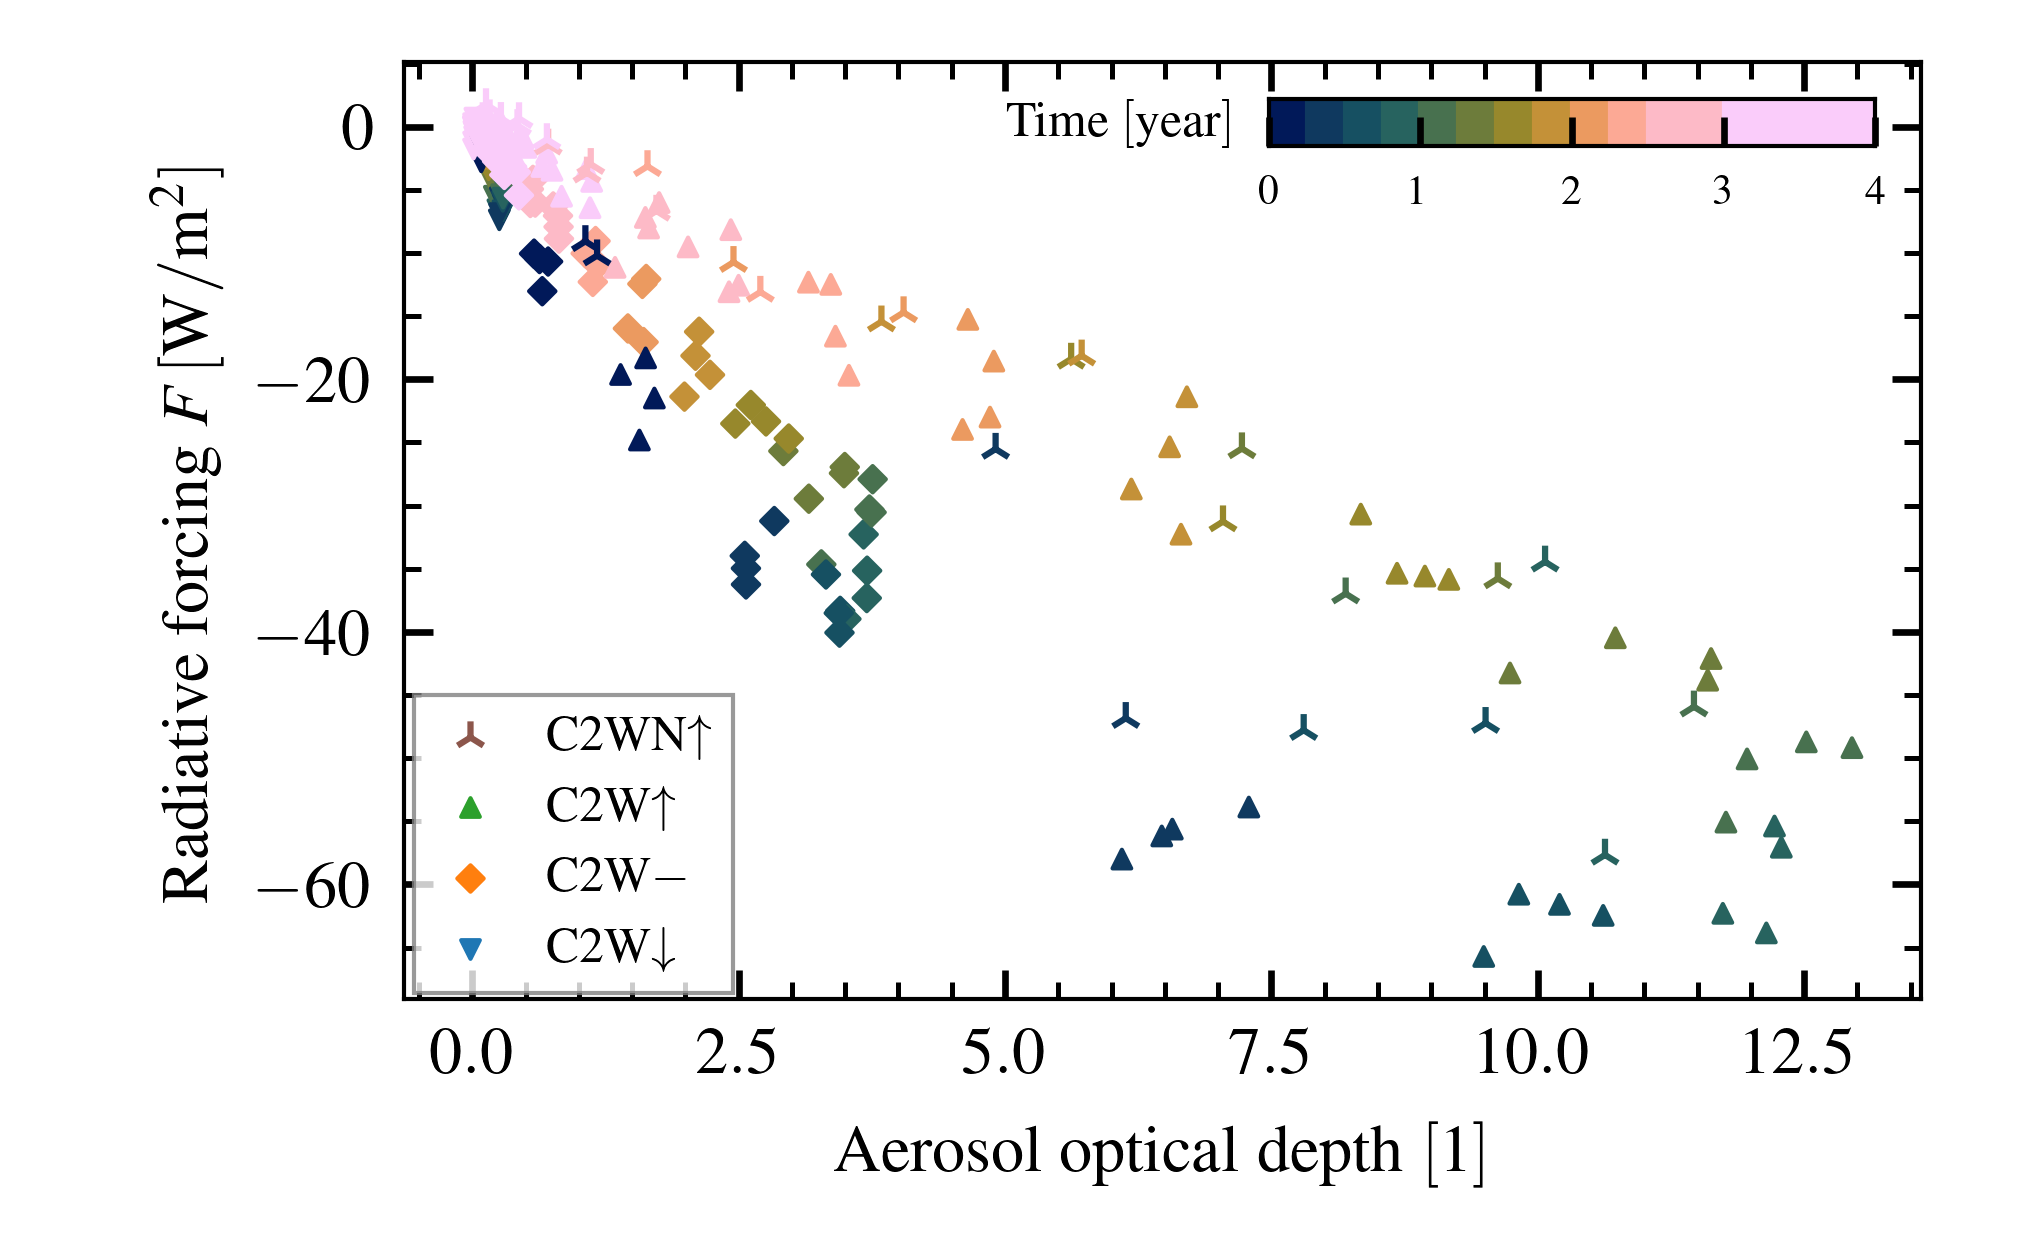
\includegraphics[width=0.95\linewidth]{figures/aod_vs_toa_avg_loop.png}
  \end{center}
  \caption{
    \acrshort{aod} versus \acrshort{toa}, with points labelled according to the
    year it was averaged from. Same type as \citet{gregory2016}
  }%
  \label{fig:aod_vs_toa_avg_loop}
\end{figure}

\begin{figure}
  \begin{center}
    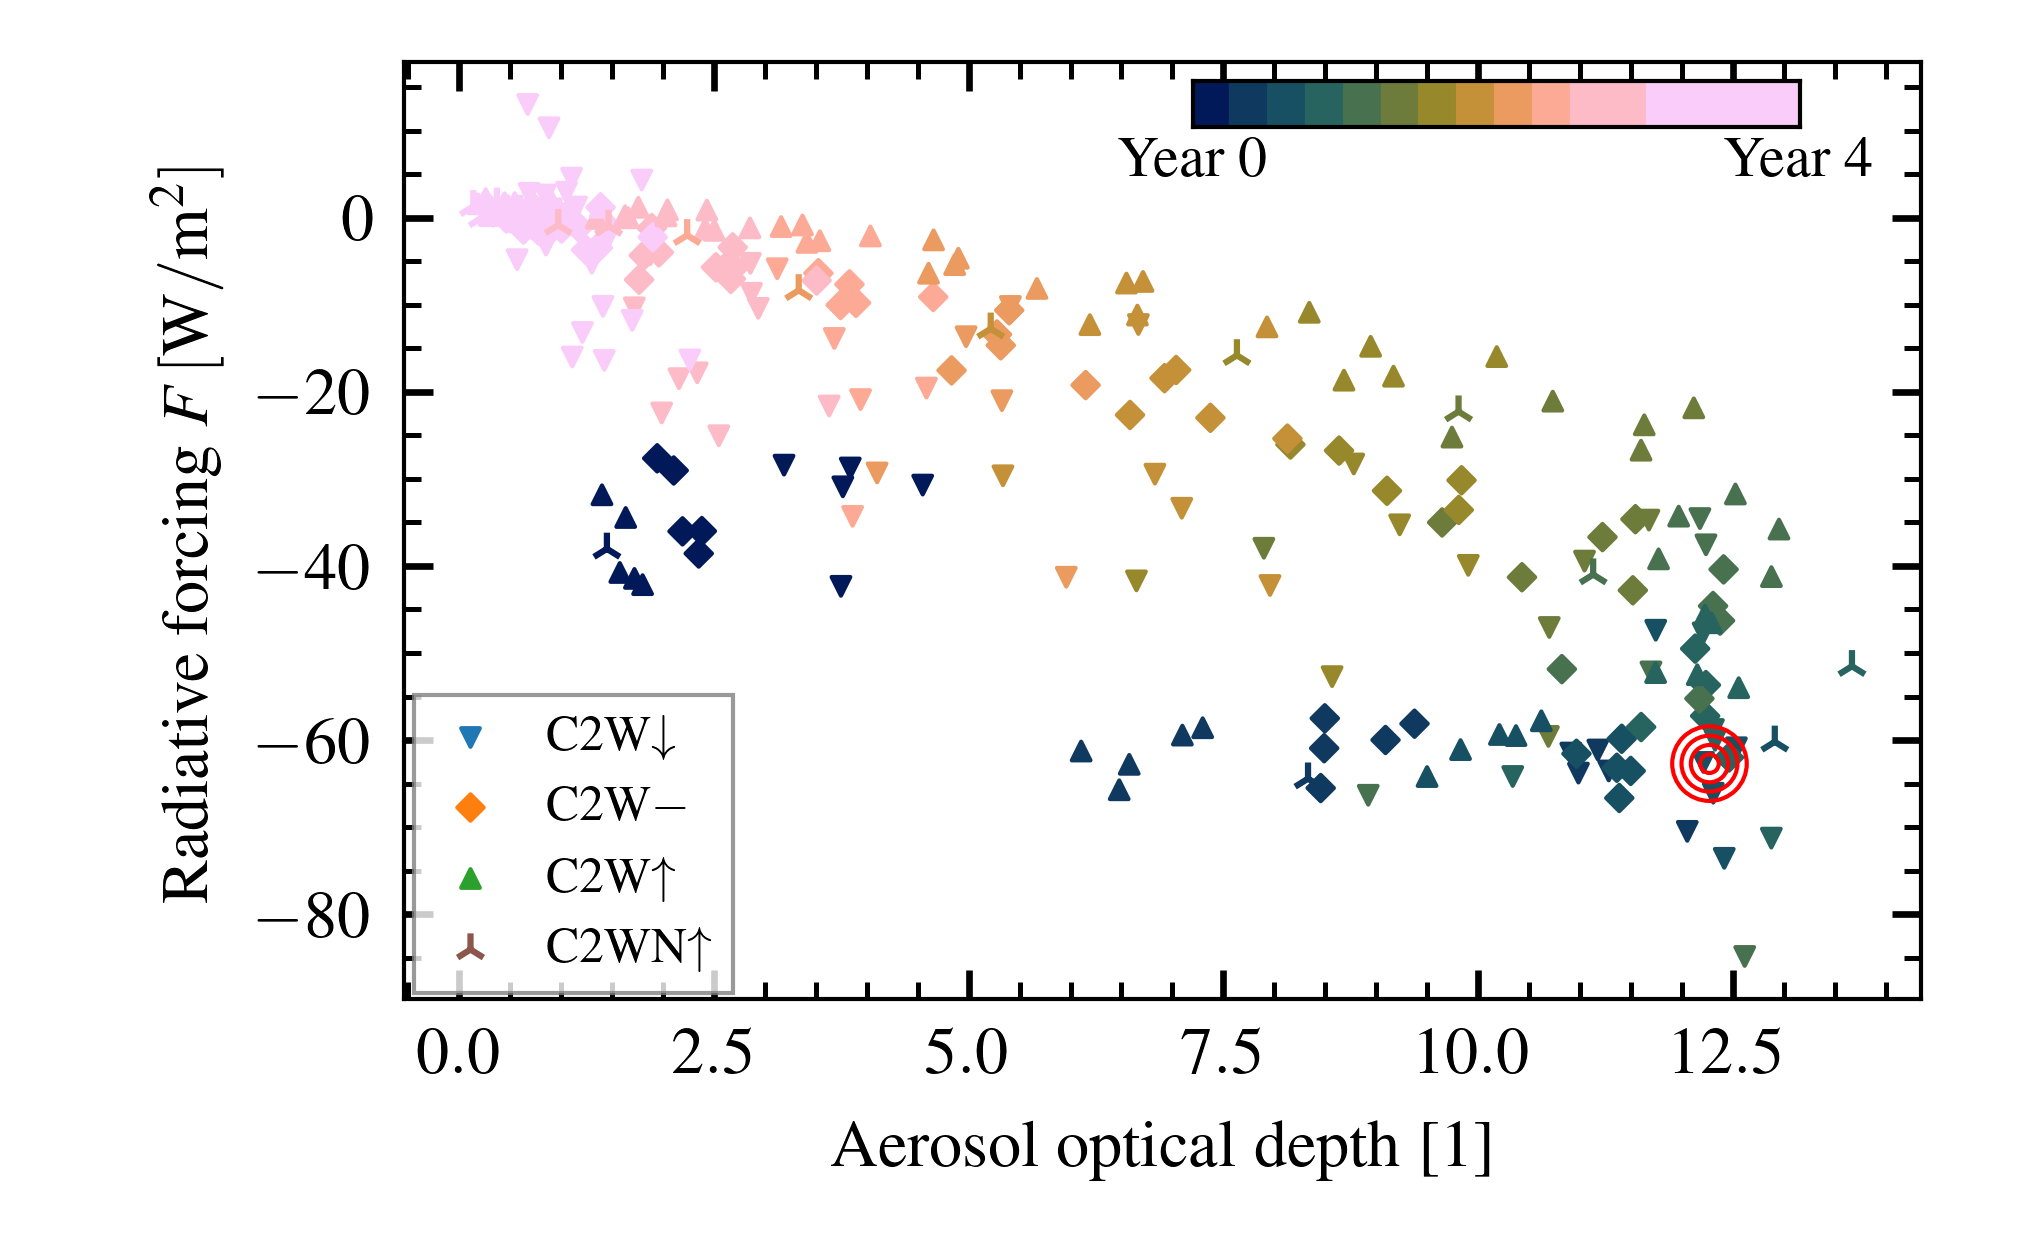
\includegraphics[width=0.95\linewidth]{figures/aod_vs_toa_avg_loop_scaled.png}
  \end{center}
  \caption{
    \acrshort{aod} versus \acrshort{toa}, with points labelled according to the
    year it was averaged from, and scaled so the peak values are aligned. Same type as
    \citet{gregory2016}
  }%
  \label{fig:aod_vs_toa_avg_loop_scaled}
\end{figure}

\begin{figure}
  \begin{center}
    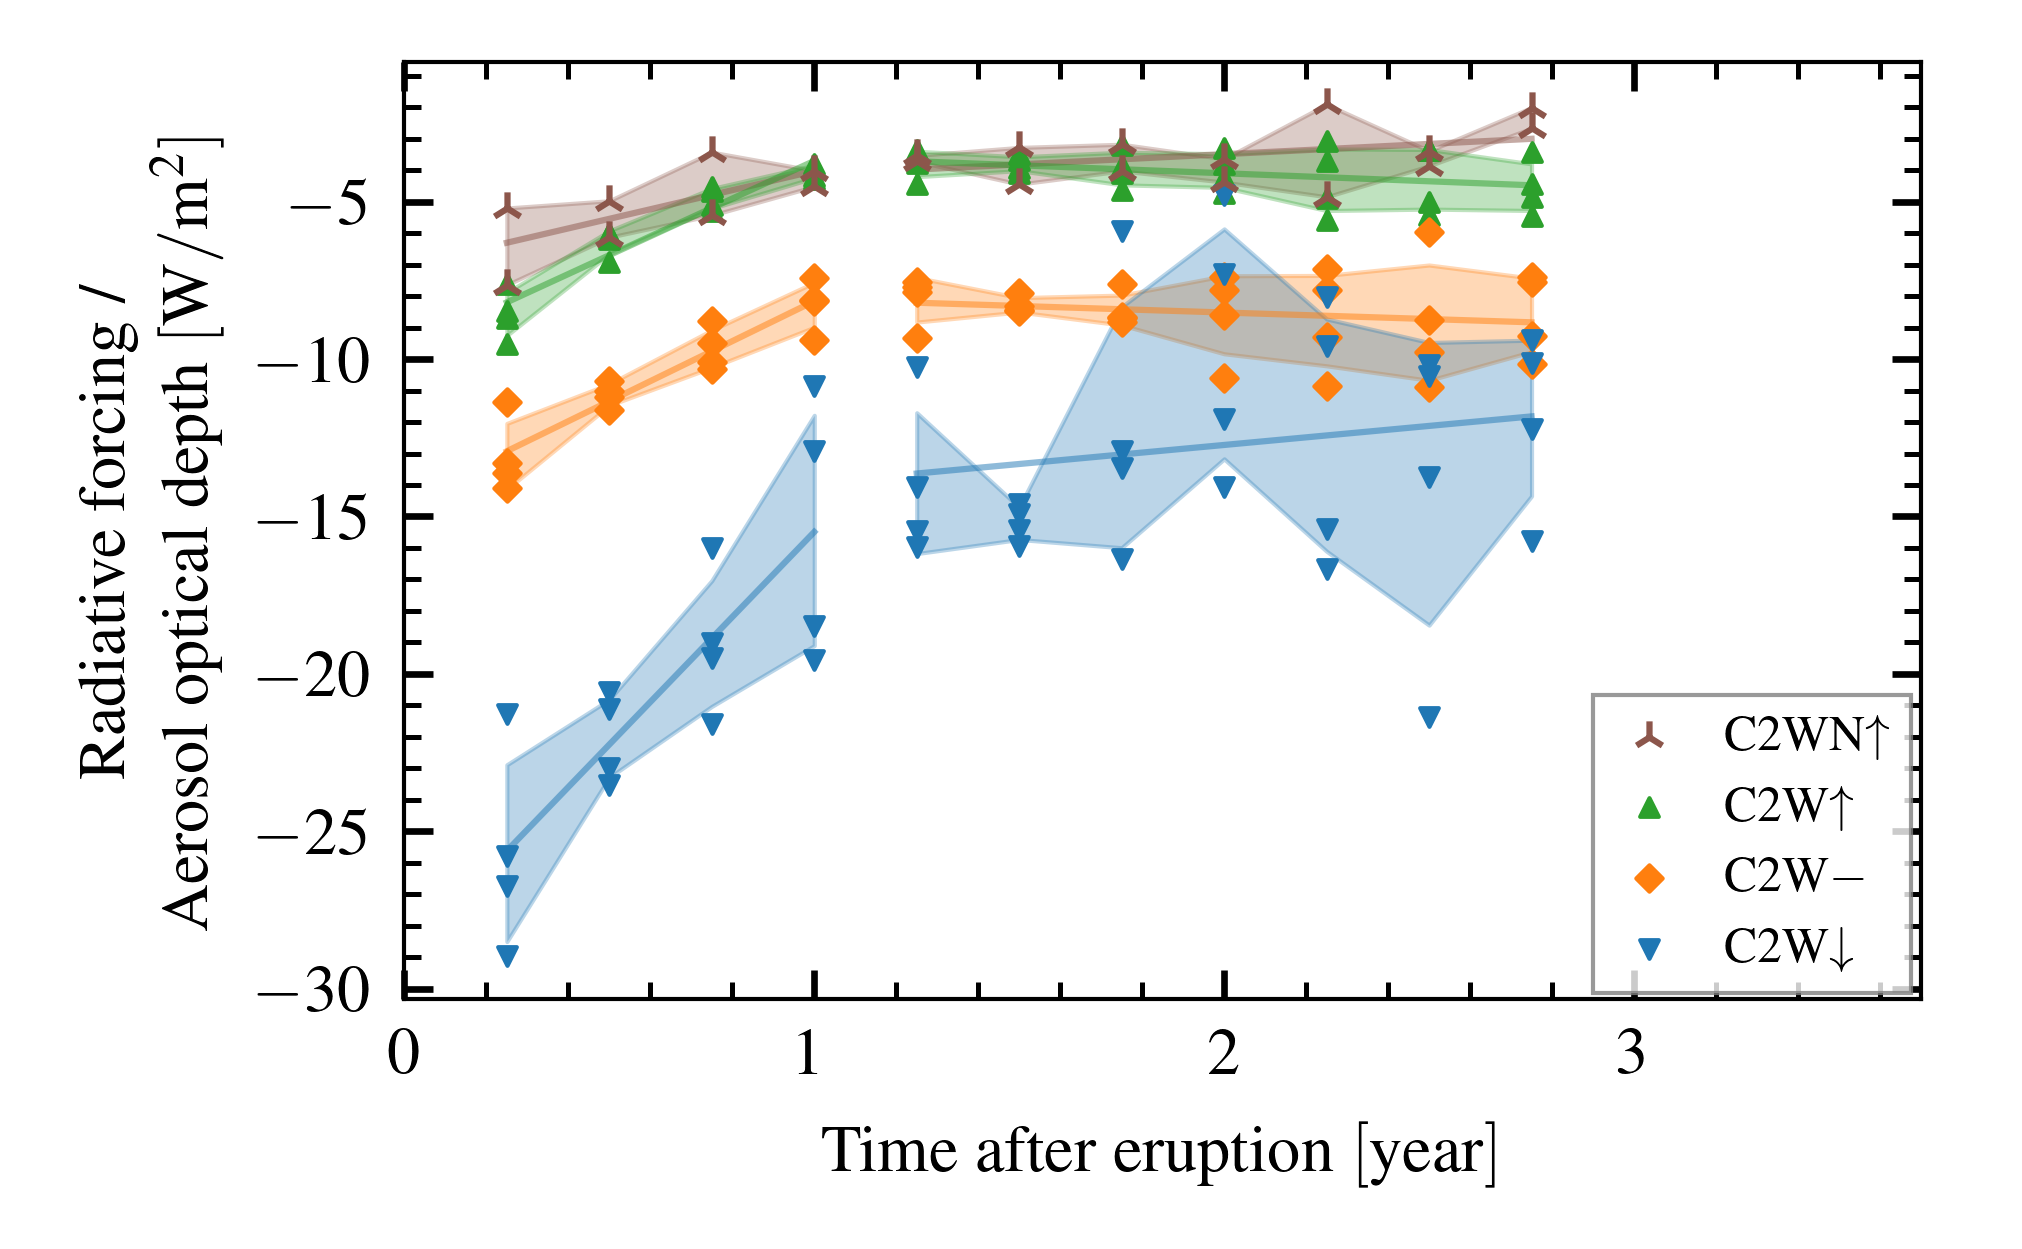
\includegraphics[width=0.95\linewidth]{figures/aod_vs_toa_avg_loop_ratio.png}
  \end{center}
  \caption{
    Ratio of \acrshort{toa} to \acrshort{aod} as shown in
    \cref{fig:aod_vs_toa_avg_loop}, with the annotated year as the horizontal axis. A
    very rough straight gradient line is included for reference, which is drawn close to
    where the most trustworthy data lies (best signal to noise ratio), with a slope of
    \(4/5\) per year
  }%
  \label{fig:aod_vs_toa_avg_loop_ratio}
\end{figure}

\begin{figure}
  \begin{center}
    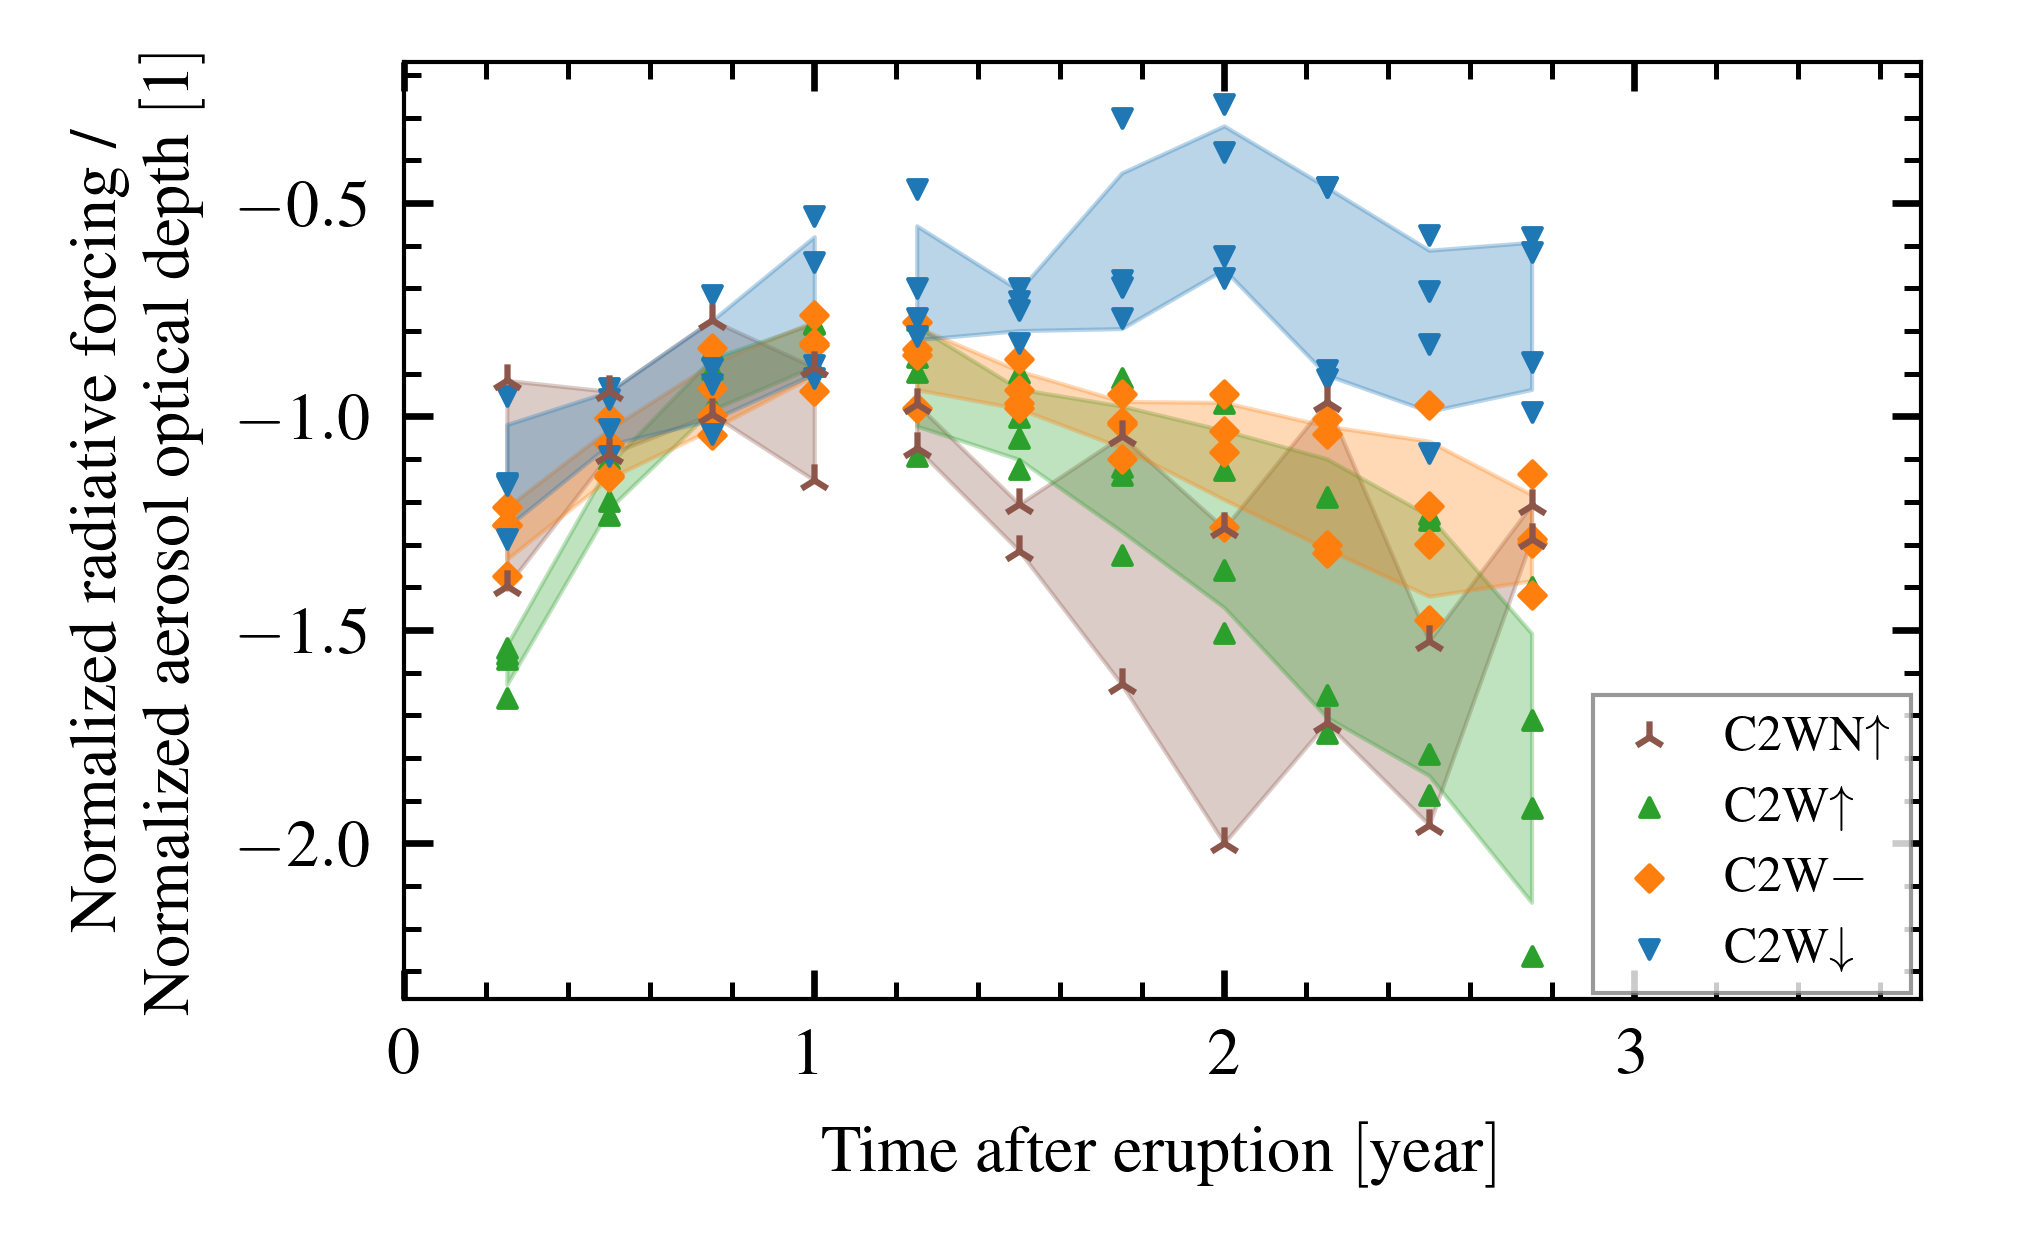
\includegraphics[width=0.95\linewidth]{figures/aod_vs_toa_avg_loop_ratio_scaled.png}
  \end{center}
  \caption{
    A scaled version of \cref{fig:aod_vs_toa_avg_loop_ratio}, where the scaling is the
    exact same as in \cref{fig:aod_vs_toa_avg_loop_scaled} compared to
    \cref{fig:aod_vs_toa_avg_loop}
  }%
  \label{fig:aod_vs_toa_avg_loop_ratio_scaled}
\end{figure}

\paragraph{Comparing parameters}

Let us now look more at different parameters that are relevant, not only \acrshort{aod}
and \acrshort{toa}. The initial parameter that is the input to the \acrshort{cesm2} is
injected \ce{SO2}. Compared to \acrshort{aod} we find that the \acrshort{cesm2}
simulations result in an almost linear relationship between them, shown in
\cref{fig:so2_vs_aod}. We do, however, find that this linear relationship only show up
the atmosphere used in the simulation is similar. One data point is from a simulation
where the low-top atmosphere \acrshort{cam6} was used (\textbf{C2C\(\uparrow\)}),
represented by the brown small star. This data point show that the \acrshort{aod} is way
smaller for the same amount of injected \ce{SO2} than what is the case with
\acrshort{waccm}. The latitude matter far less than the model complexity, as we can see
from the \textbf{C2WN\(\uparrow\)} data point, representing a strong eruption similar to
the strong eruption from before, but located at \( \SI{56}{\degree N} \). The weak
dependence on eruption latitude is also reported in \citet{marshall2019}.

\begin{figure}
  \begin{center}
    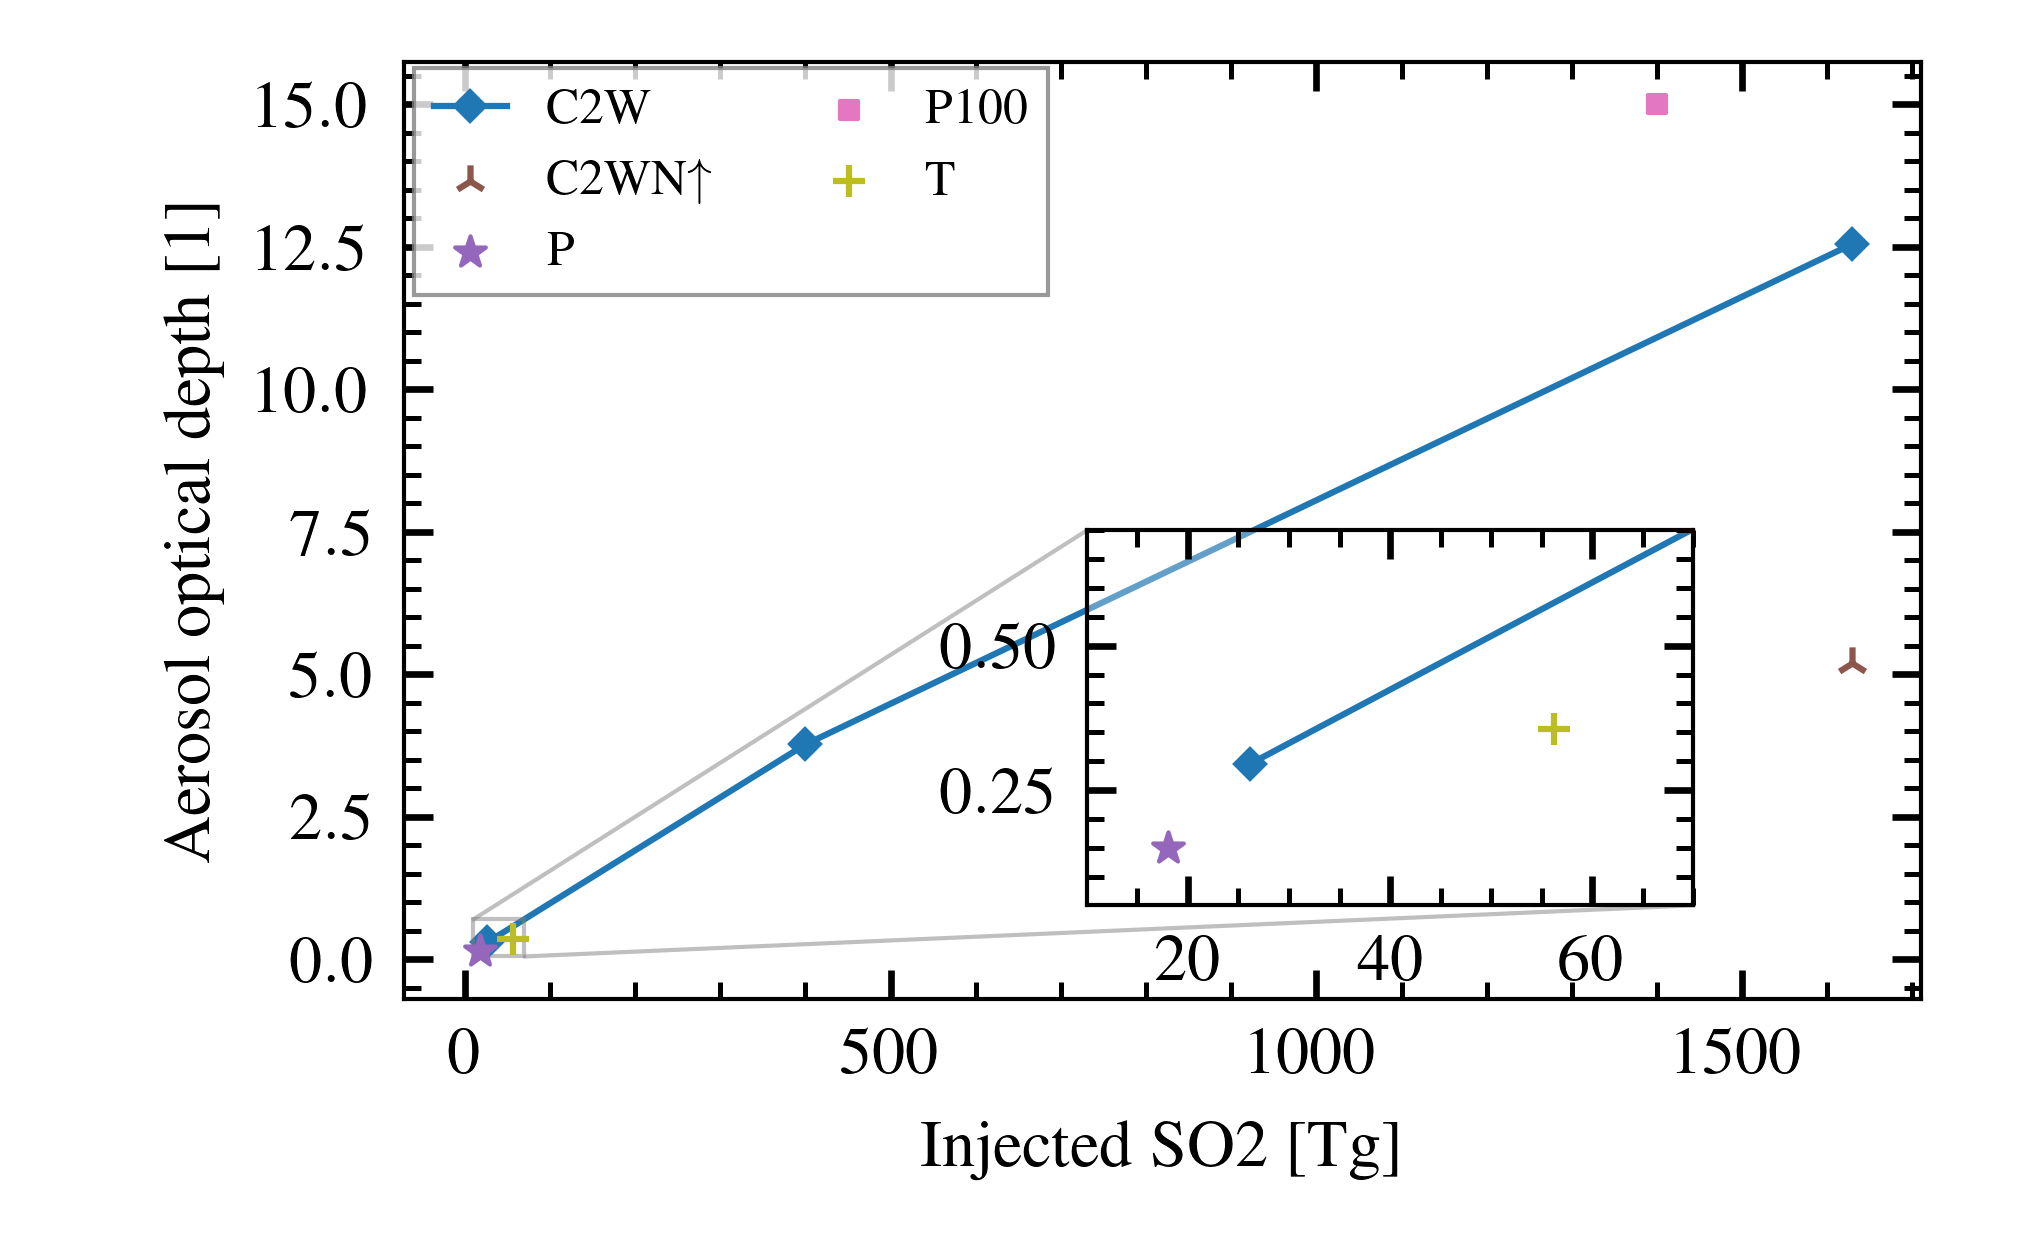
\includegraphics[width=0.95\linewidth]{figures/injection_vs_aod.png}
  \end{center}
  \caption{Injected \ce{SO2} versus \acrshort{aod}}%
  \label{fig:so2_vs_aod}
\end{figure}

With the almost linear relation between injected \ce{SO2} and \acrshort{aod}, we should
expect to see a similar plot for \iso{} versus \acrshort{toa} as for \acrshort{aod}
versus \acrshort{toa}. \iso[I] versus \acrshort{toa} is shown in \cref{fig:so2_vs_toa},
but where the absolute value of the \acrshort{toa} is potted along the \( y \)-axis
instead of the true value. Just as in \cref{fig:aod_vs_toa_full} we find the
\acrshort{cesm2} data points to be heavily damped in \acrshort{toa} compared to \iso.
The same effect can be seen in the data from \citet{ottobliesner2016} (labelled
\textbf{C1C}, red points), but here the \acrshort{toa} keeps up at larger values for
longer. The simulations used by \citet{ottobliesner2016} was with \acrshort{cesm} as
well, but version 1 (\acrshort{cesm1}) and with a low-top atmosphere (\acrshort{cam5}),
which makes it more comparable to our \textbf{C2C\(\uparrow\)} simulation. However, due
to the very small \acrshort{aod} values this gave (\cref{fig:so2_vs_aod}) we would not
expect the \acrshort{cam6} simulation to have greater \acrshort{toa} than the
\acrshort{waccm} simulations.

\begin{figure}
  \begin{center}
    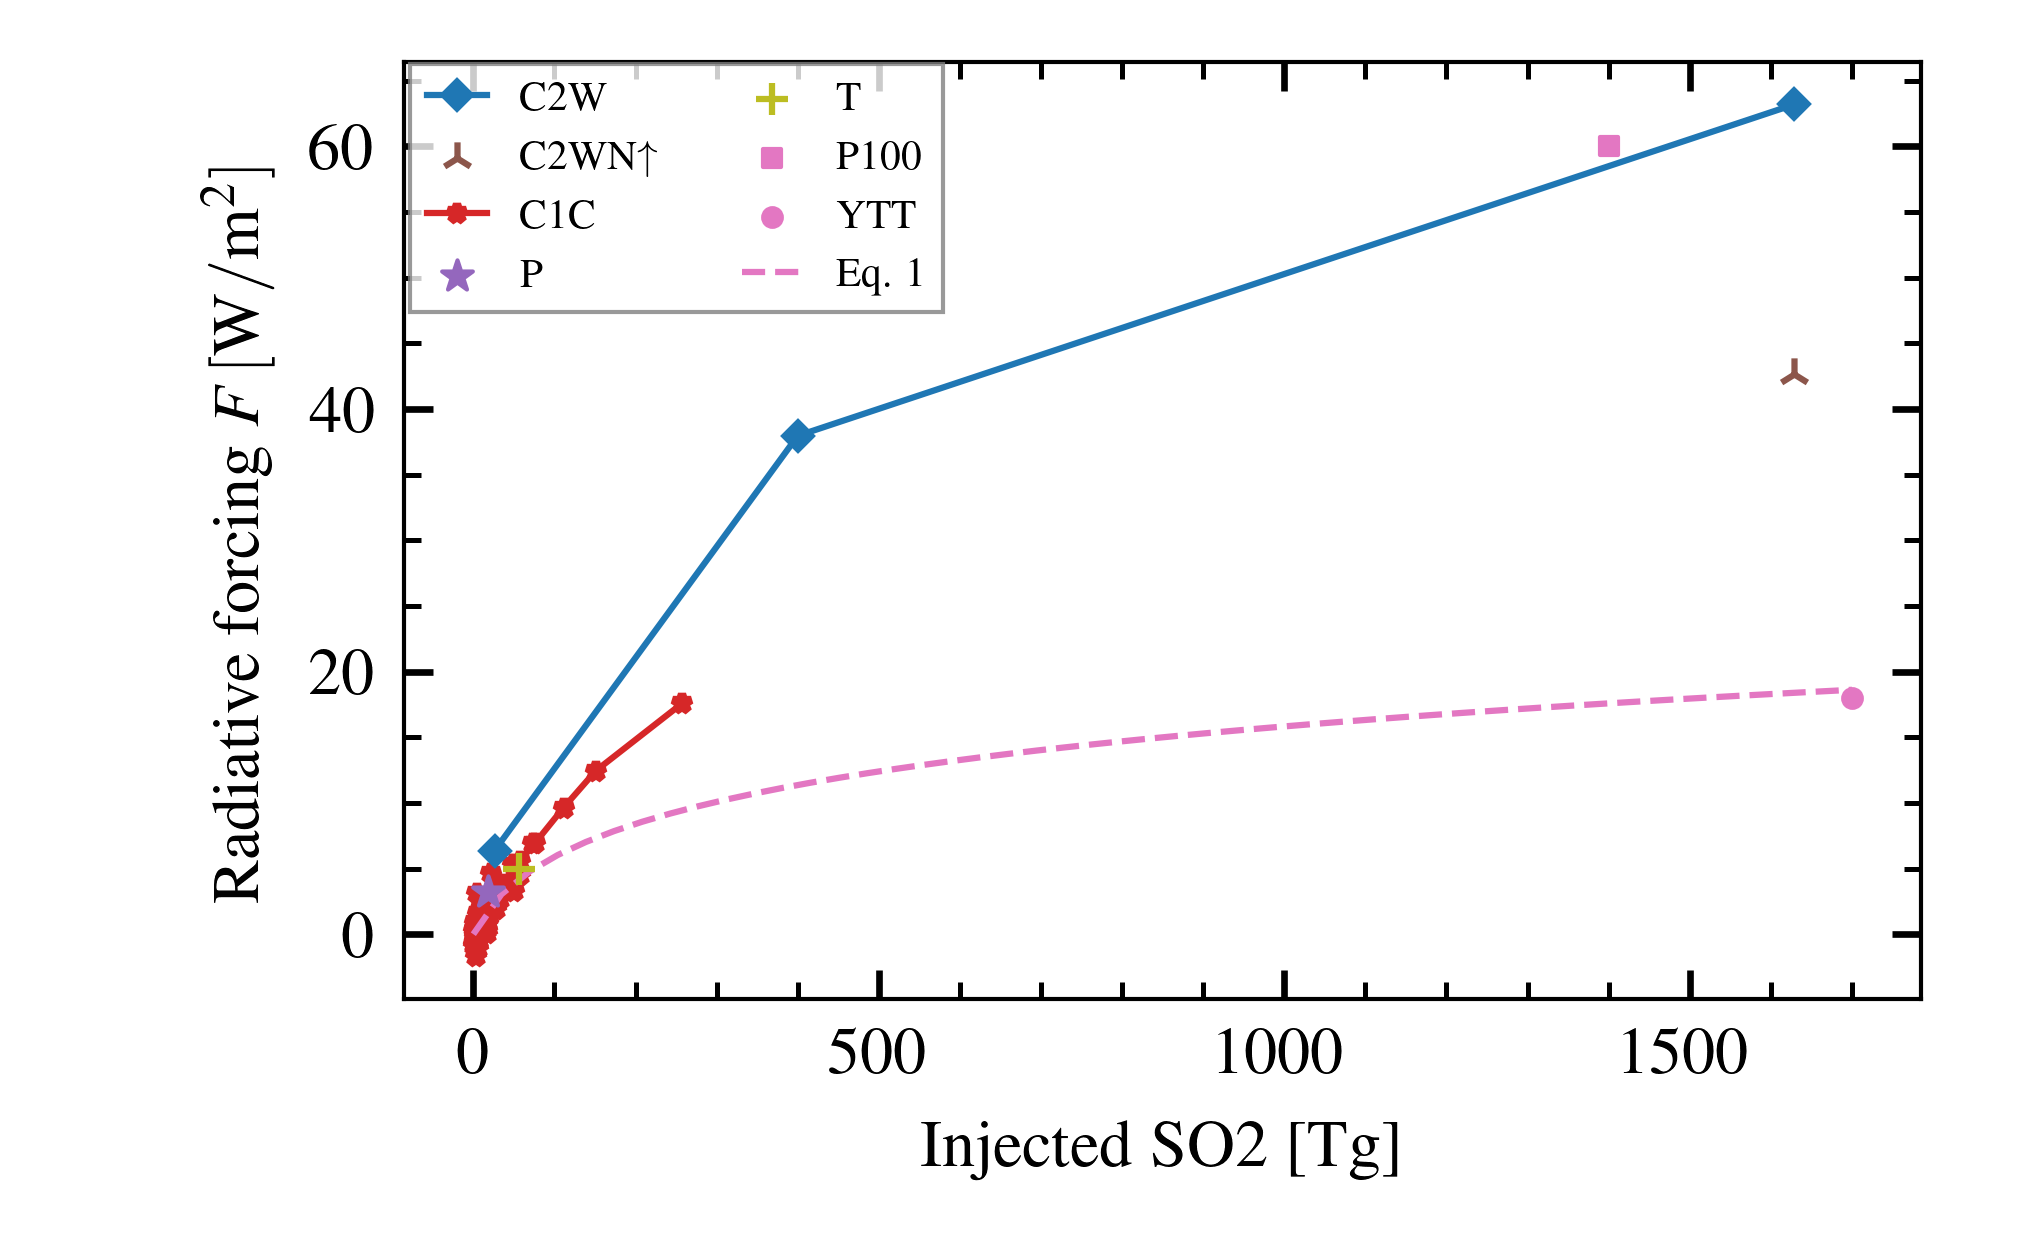
\includegraphics[width=0.95\linewidth]{figures/injection_vs_toa.png}
  \end{center}
  \caption{Injected \ce{SO2} versus \acrshort{toa} radiative imbalance}%
  \label{fig:so2_vs_toa}
\end{figure}

\Cref{fig:so2_vs_temp} show \iso{} versus temperature response. Just as in
\cref{fig:so2_vs_toa}, the points from the \acrshort{cesm2} simulations bend off, making
the temperature response less extreme for higher values of \iso. Again we see that the
data from the \acrshort{cesm1} simulations by \citet{ottobliesner2016} follow a
different path than the \acrshort{cesm2} data, likely cased by the different atmospheres
being used.

\begin{figure}
  \begin{center}
    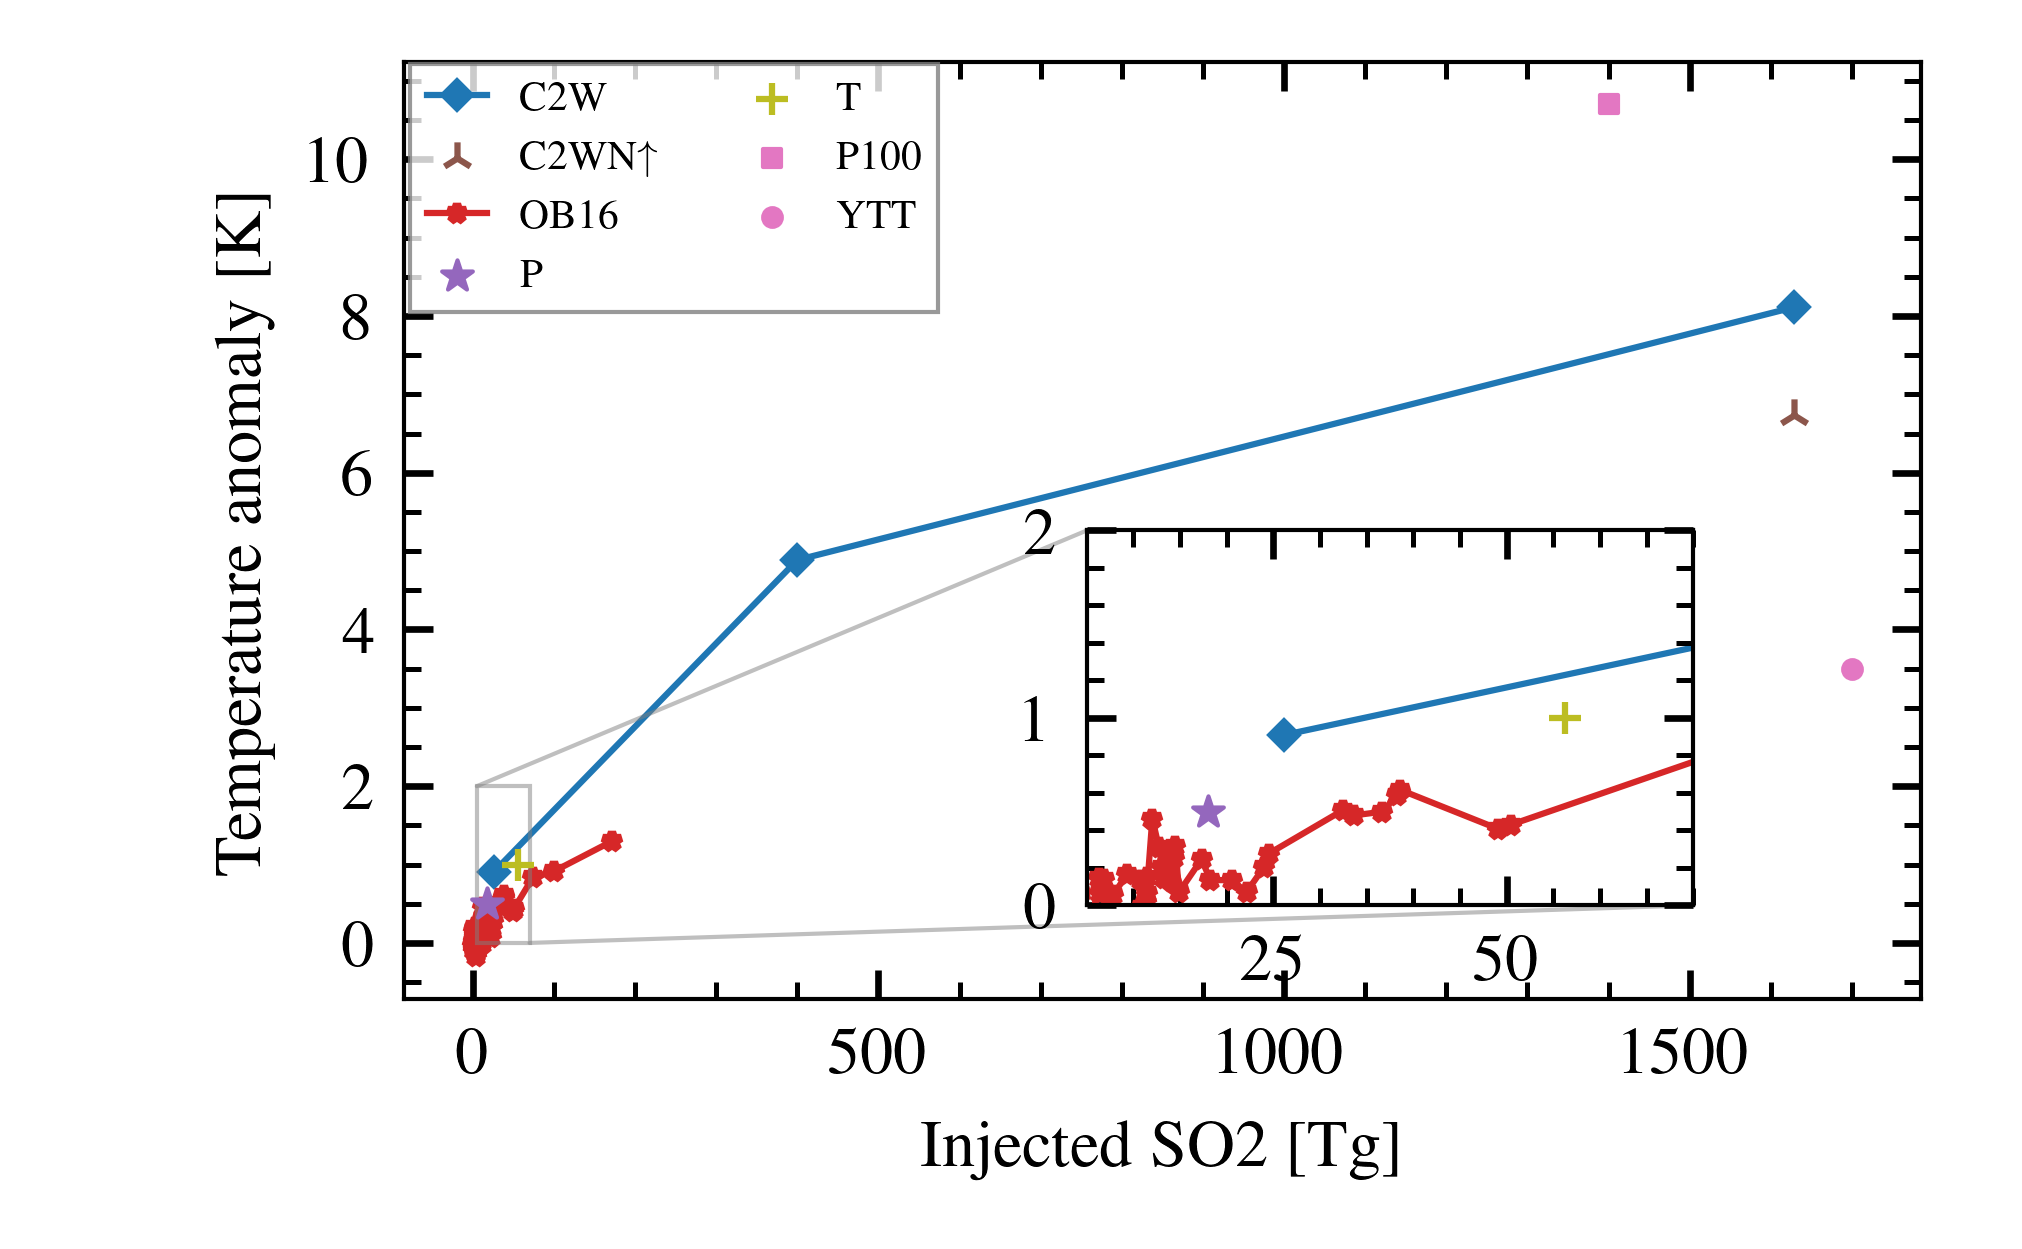
\includegraphics[width=0.95\linewidth]{figures/injection_vs_temperature.png}
  \end{center}
  \caption{Injected \ce{SO2} versus temperature}%
  \label{fig:so2_vs_temp}
\end{figure}

\Cref{fig:aod_vs_temp} should in the case of the \acrshort{cesm2} data points be very
similar in shape to the paths found in \cref{fig:so2_vs_temp}, and this is indeed what
we find. The relationship between \acrshort{aod} and temperature is slightly more linear
than what is the case with \iso{} and temperature, but the tendency is the same, as one
would expect based on the close to linear relationship found between \iso{} and
\acrshort{aod} in \cref{fig:so2_vs_aod}.

\begin{figure}
  \begin{center}
    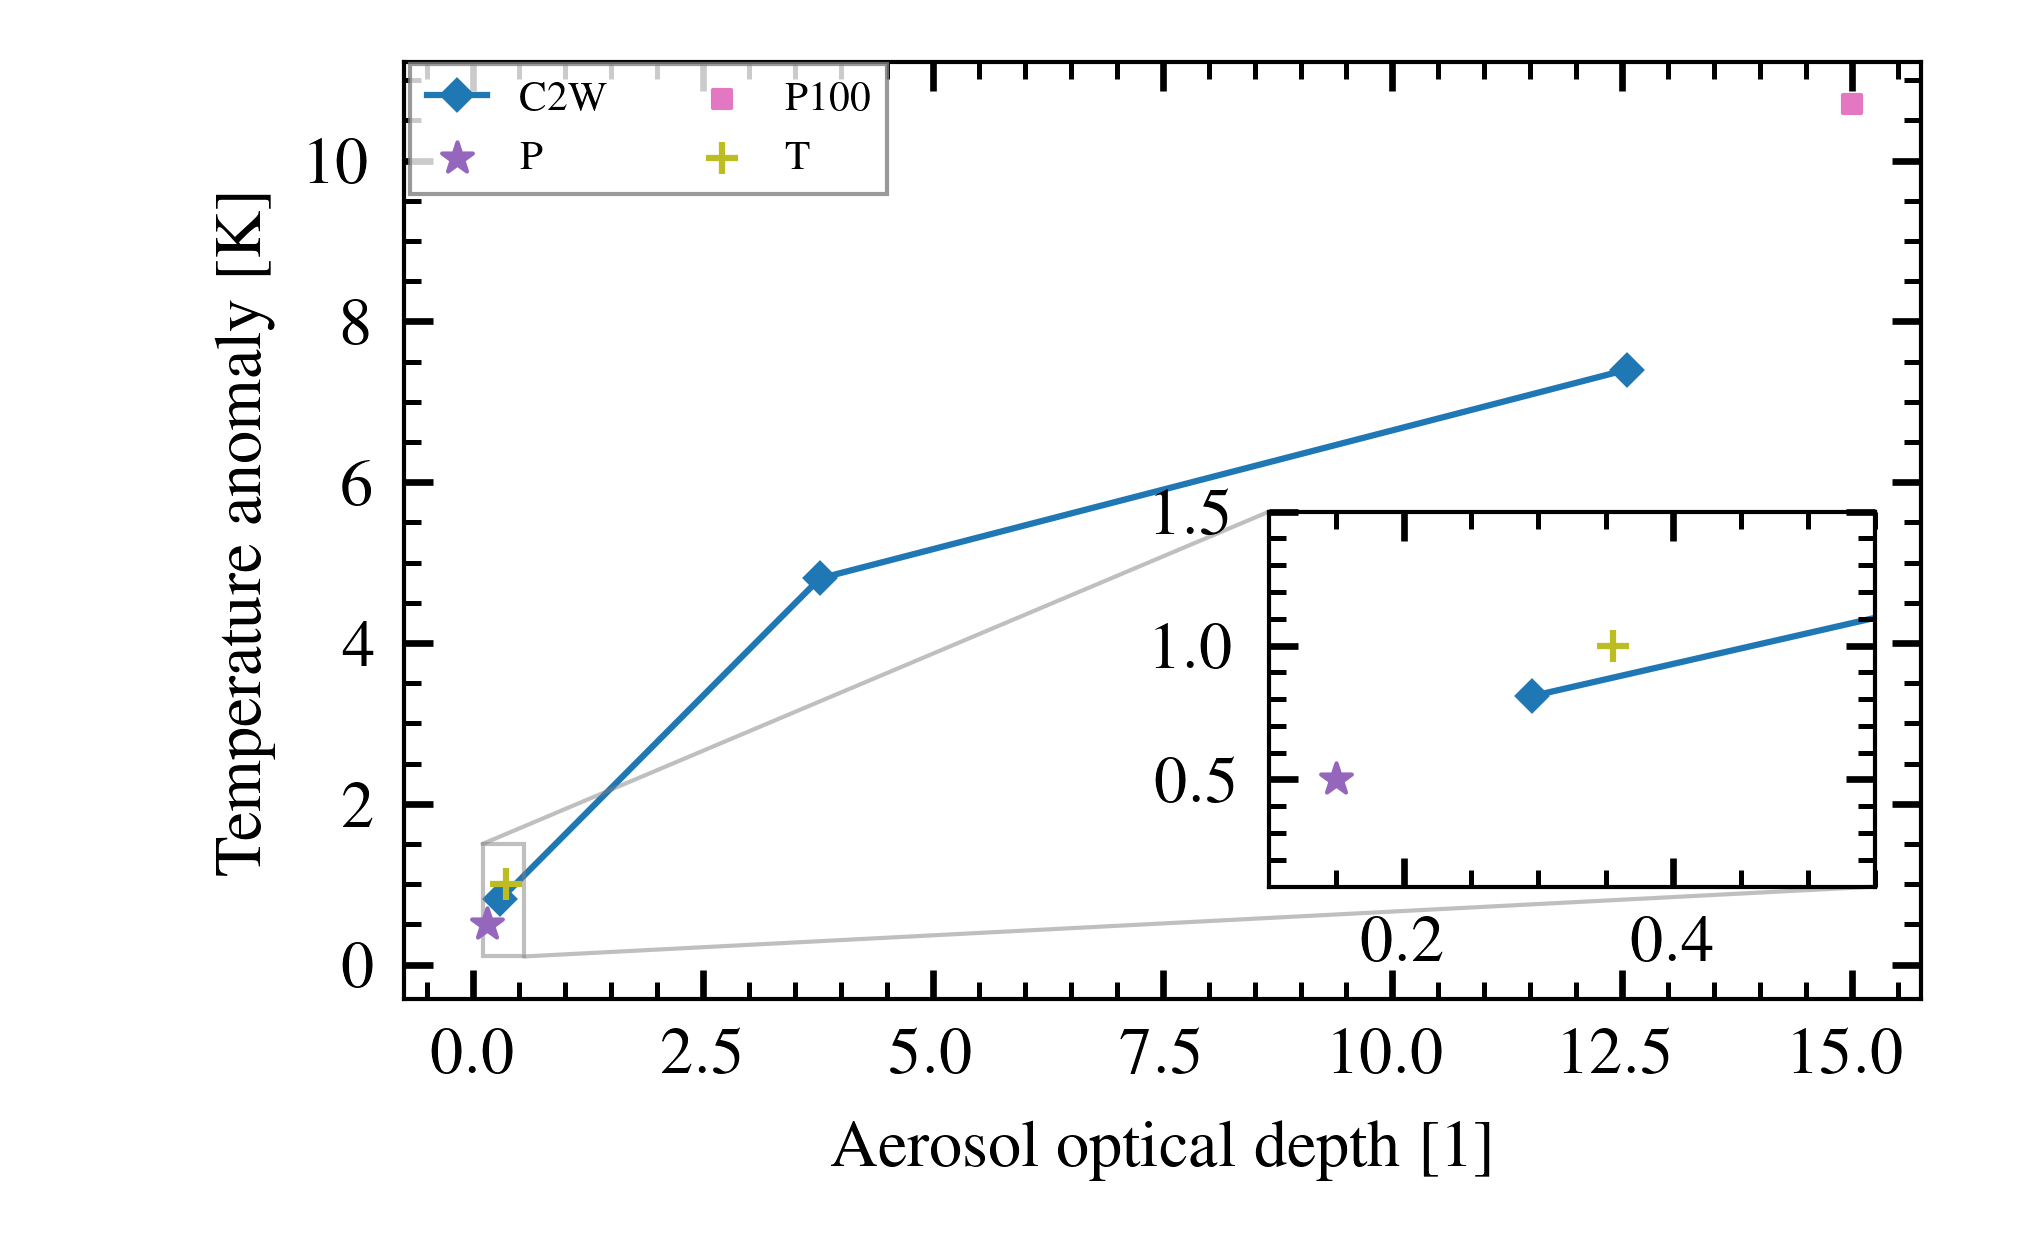
\includegraphics[width=0.95\linewidth]{figures/aod_vs_temperature.png}
  \end{center}
  \caption{\acrshort{aod} versus temperature}%
  \label{fig:aod_vs_temp}
\end{figure}

In \cref{fig:toa_vs_temp} we compare the \acrshort{toa}, usually what is referred to
when talking about forcing, and temperature response. There is a tendency that the
temperature response is stronger as the radiative forcing increases, or that the forcing
is more efficient the stringer it is, when inspecting the \acrshort{cesm2} data. The
corresponding data from \citet{ottobliesner2016} coming out of \acrshort{cesm1} show a
much more linear relationship, and also temperature responses that are much weaker for a
given forcing than what we get from \acrshort{cesm2}. (Might change as we update the
fSST simulation).

\begin{figure}
  \begin{center}
    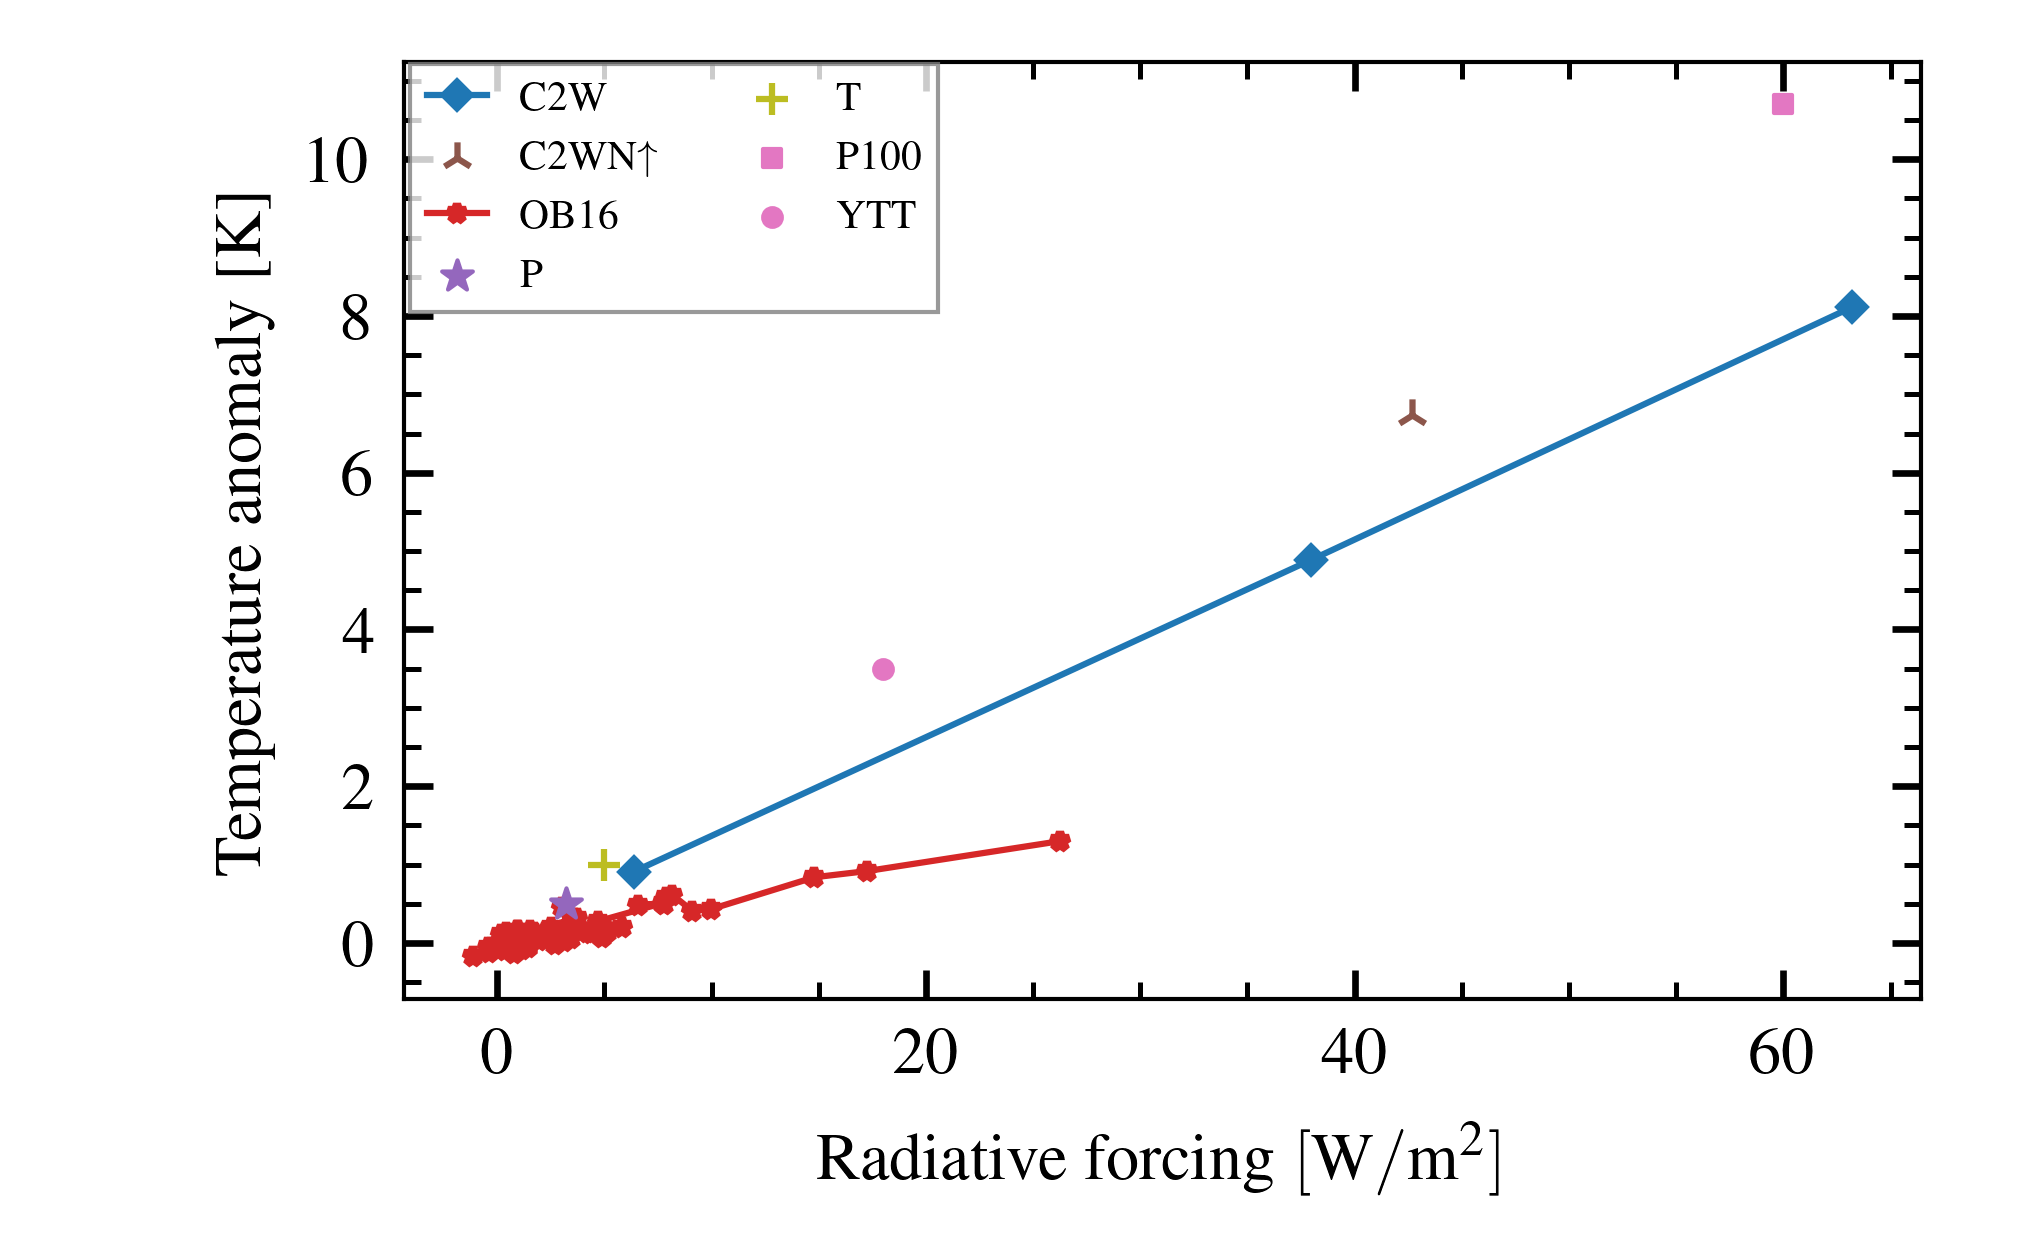
\includegraphics[width=0.95\linewidth]{figures/toa_vs_temperature.png}
  \end{center}
  \caption{\acrshort{toa} versus temperature}%
  \label{fig:toa_vs_temp}
\end{figure}

\clearpage

% %%%%%%%%%%%%%%%%%%%%%%%%%%%%%%%%%%%%%%%%%%%%%%%%%%%%%%%%%%%%%%%%%%%%%%%%%%%%%%%%%%%%%%
% ACKNOWLEDGMENTS
% %%%%%%%%%%%%%%%%%%%%%%%%%%%%%%%%%%%%%%%%%%%%%%%%%%%%%%%%%%%%%%%%%%%%%%%%%%%%%%%%%%%%%%
% \acknowledgments

% Keep acknowledgments (note correct spelling: no ``e'' between the ``g'' and ``m'') as
% brief as possible. In general, acknowledge only direct help in writing or research.
% Financial support (e.g., grant numbers) for the work done, for an author, or for the
% laboratory where the work was performed is best acknowledged here rather than as
% footnotes to the title or to an author's name. Contribution numbers (if the work has
% been published by the author's institution or organization) should be included as
% footnotes on the title page, not in the acknowledgments.

% %%%%%%%%%%%%%%%%%%%%%%%%%%%%%%%%%%%%%%%%%%%%%%%%%%%%%%%%%%%%%%%%%%%%%%%%%%%%%%%%%%%%%%
% DATA AVAILABILITY STATEMENT
% %%%%%%%%%%%%%%%%%%%%%%%%%%%%%%%%%%%%%%%%%%%%%%%%%%%%%%%%%%%%%%%%%%%%%%%%%%%%%%%%%%%%%%
% \datastatement

% The data availability statement is where authors should describe how the data
% underlying the findings within the article can be accessed and reused. Authors should
% attempt to provide unrestricted access to all data and materials underlying reported
% findings. If data access is restricted, authors must mention this in the statement.

% %%%%%%%%%%%%%%%%%%%%%%%%%%%%%%%%%%%%%%%%%%%%%%%%%%%%%%%%%%%%%%%%%%%%%%%%%%%%%%%%%%%%%%
% APPENDIXES
% %%%%%%%%%%%%%%%%%%%%%%%%%%%%%%%%%%%%%%%%%%%%%%%%%%%%%%%%%%%%%%%%%%%%%%%%%%%%%%%%%%%%%%
%
% Use \appendix if there is only one appendix.
% \appendix

% Use \appendix[A], \appendix[B], if you have multiple appendixes.
% \appendix[A]

% Appendix title is necessary! For appendix title:
% \appendixtitle{}

% Appendix section numbering (note, skip \section and begin with \subsection)
% \subsection{First primary heading}

% \subsubsection{First secondary heading}

% \paragraph{First tertiary heading}

% Important!
% \appendcaption{<appendix letter and number>}{<caption>}
% must be used for figures and tables in appendixes, e.g.,
%
% \begin{figure}
% \noindent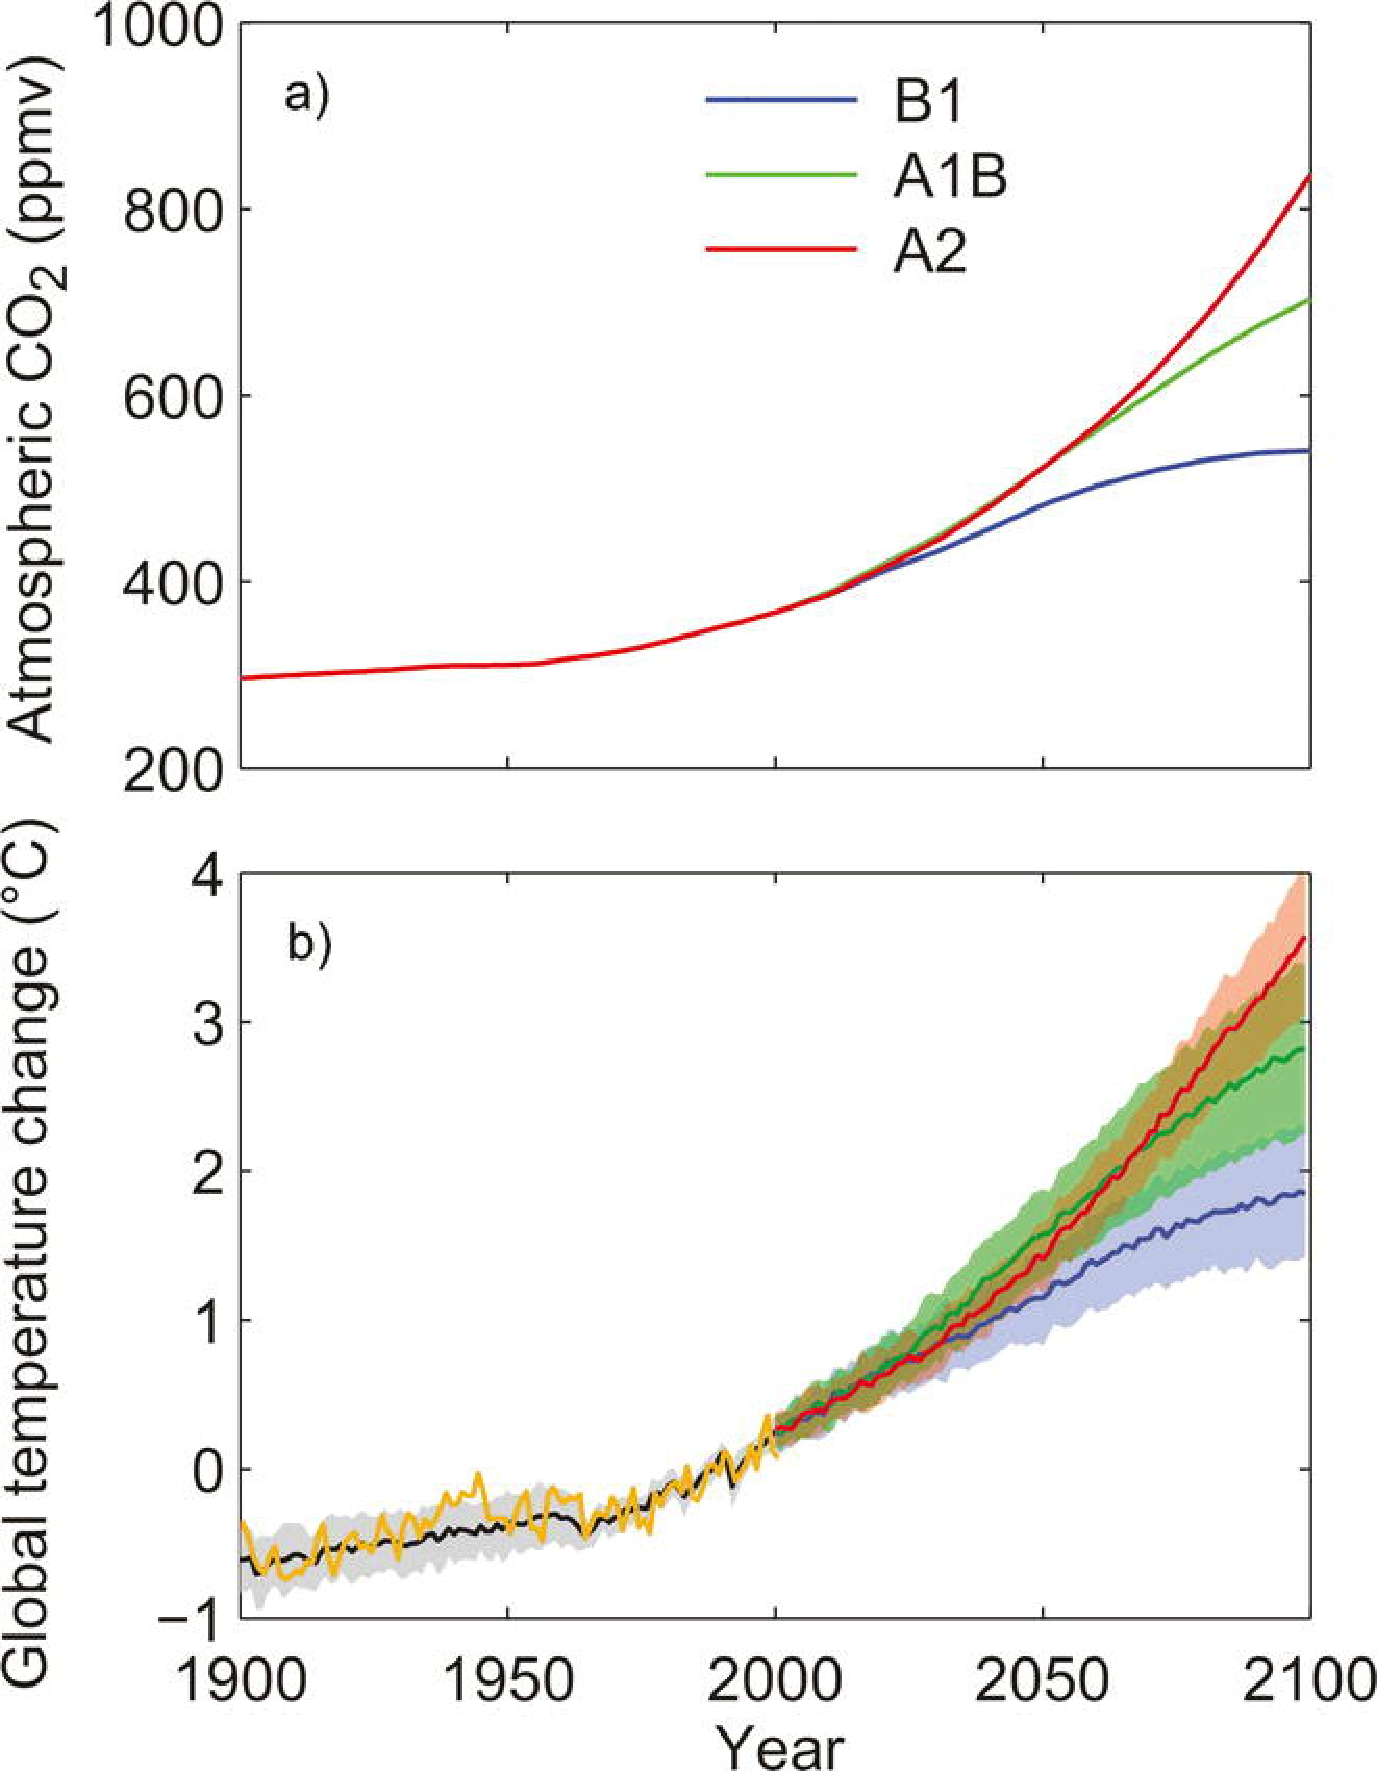
\includegraphics[width=19pc,angle=0]{figure01.pdf}\\
% \appendcaption{A1}{Caption here.}
% \end{figure}
%
% All appendix figures/tables should be placed in order AFTER the main figures/tables,
% i.e., tables, appendix tables, figures, appendix figures.
%
% %%%%%%%%%%%%%%%%%%%%%%%%%%%%%%%%%%%%%%%%%%%%%%%%%%%%%%%%%%%%%%%%%%%%%%%%%%%%%%%%%%%%%%
% REFERENCES
% %%%%%%%%%%%%%%%%%%%%%%%%%%%%%%%%%%%%%%%%%%%%%%%%%%%%%%%%%%%%%%%%%%%%%%%%%%%%%%%%%%%%%%
% Make your BibTeX bibliography by using these commands:
\bibliographystyle{ametsoc2014}
\bibliography{references}
\clearpage
\printglossary[type=\acronymtype,title=List of Acronyms]
% %%%%%%%%%%%%%%%%%%%%%%%%%%%%%%%%%%%%%%%%%%%%%%%%%%%%%%%%%%%%%%%%%%%%%%%%%%%%%%%%%%%%%%
% TABLES
% %%%%%%%%%%%%%%%%%%%%%%%%%%%%%%%%%%%%%%%%%%%%%%%%%%%%%%%%%%%%%%%%%%%%%%%%%%%%%%%%%%%%%%
% Enter tables at the end of the document, before figures.
%
% \begin{table}[t]
%   \caption{This is a sample table caption and table layout.  Enter as many tables as
%     necessary at the end of your manuscript. Table from Lorenz (1963).}\label{t1}
%   \begin{center}
%     \begin{tabular}{ccccrrcrc}
%       \hline\hline
%       $N$  & $X$  & $Y$  & $Z$  \\
%       \hline
%       0000 & 0000 & 0010 & 0000 \\
%       0005 & 0004 & 0012 & 0000 \\
%       0010 & 0009 & 0020 & 0000 \\
%       0015 & 0016 & 0036 & 0002 \\
%       0020 & 0030 & 0066 & 0007 \\
%       0025 & 0054 & 0115 & 0024 \\
%       \hline
%     \end{tabular}
%   \end{center}
% \end{table}

% %%%%%%%%%%%%%%%%%%%%%%%%%%%%%%%%%%%%%%%%%%%%%%%%%%%%%%%%%%%%%%%%%%%%%%%%%%%%%%%%%%%%%%
% FIGURES
% %%%%%%%%%%%%%%%%%%%%%%%%%%%%%%%%%%%%%%%%%%%%%%%%%%%%%%%%%%%%%%%%%%%%%%%%%%%%%%%%%%%%%%
% Enter figures at the end of the document, after tables.
%
% \begin{figure}[t]
%   \noindent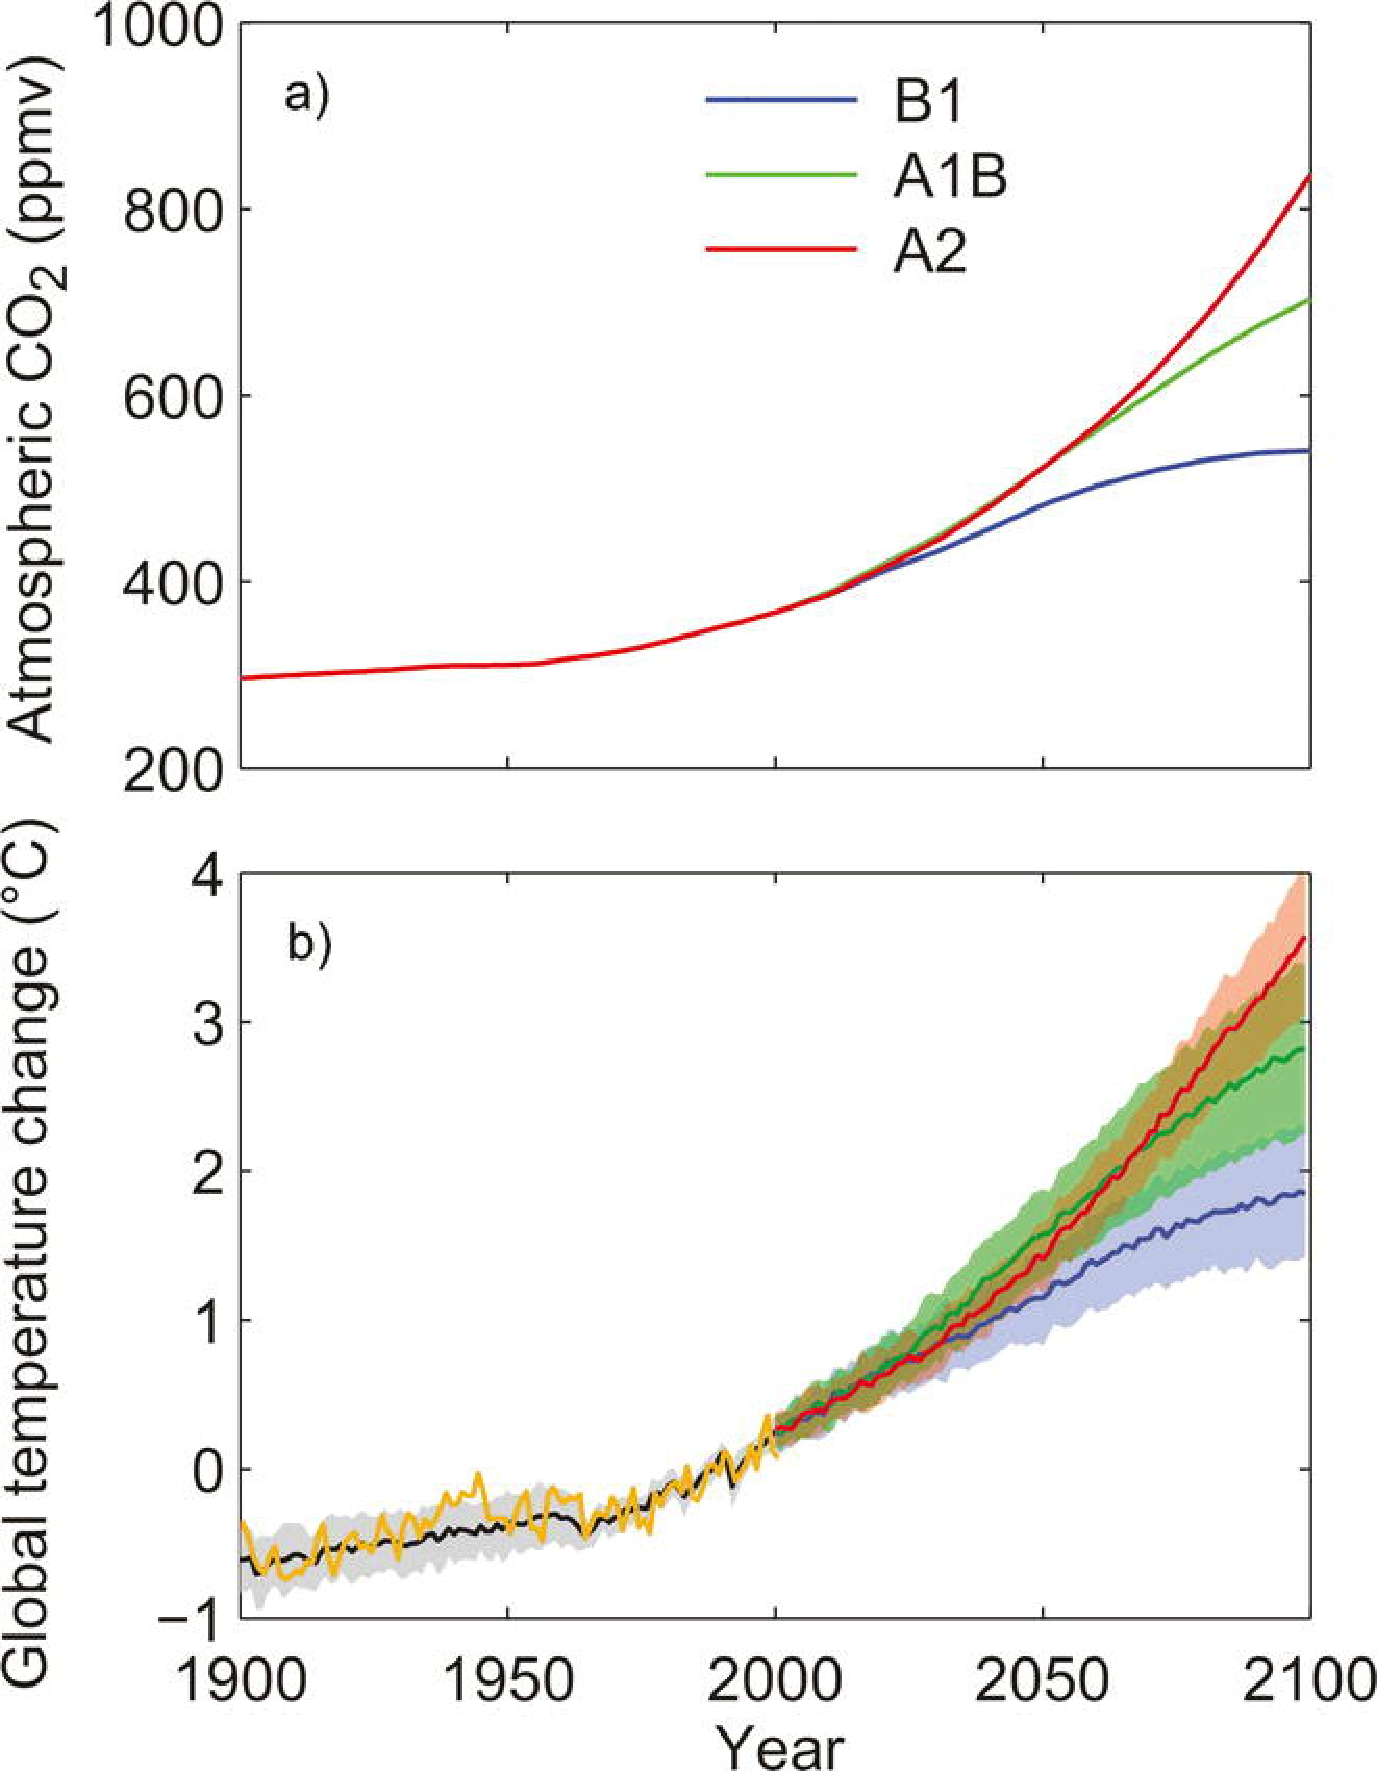
\includegraphics[width=19pc,angle=0]{figure01.pdf}\\
%   \caption{Enter the caption for your figure here.  Repeat as
%     necessary for each of your figures. Figure from \protect\cite{Knutti2008}.}\label{f1}
% \end{figure}

\end{document}
